% =====================================================================
%  Rapport de projet — Modern Data Platform WWI & Text-to-SQL Cortex AI
%  Compilation : pdflatex rapport.tex (deux fois, pour la table des matières)
% =====================================================================
\documentclass[11pt,a4paper,oneside]{report}

% ---------------------------------------------------------------- informations
\newcommand{\auteur}{Mouhamed DIOP}
\newcommand{\encadrant}{Dr Jean Gane SARR}
\newcommand{\anneeuniv}{2025 -- 2026}
\newcommand{\titreprojet}{Conception d'une Modern Data Platform avec architecture Médaillon et développement d'une application Text-to-SQL basée sur l'IA}

% ---------------------------------------------------------------- paquets
\usepackage[T1]{fontenc}
\usepackage[utf8]{inputenc}
\usepackage[french]{babel}
\usepackage{lmodern}
\usepackage{microtype}
\usepackage[a4paper,margin=2.5cm,headheight=14pt]{geometry}
\usepackage{graphicx}
\usepackage{xcolor}
\usepackage{booktabs}
\usepackage{tabularx}
\usepackage{longtable}
\usepackage{array}
\usepackage{multirow}
\usepackage{enumitem}
\usepackage{caption}
\usepackage{float}
\usepackage{fancyhdr}
\usepackage{titlesec}
\usepackage{listings}
\usepackage{tcolorbox}
\usepackage{tikz}
\usetikzlibrary{arrows.meta,positioning,shapes.geometric,shapes.multipart,fit,backgrounds,calc,shadows}
\usepackage[hidelinks]{hyperref}
\usepackage{csquotes}

% ---------------------------------------------------------------- couleurs
\definecolor{ucadblue}{HTML}{1F8FD8}
\definecolor{ucaddark}{HTML}{0B3C5D}
\definecolor{bronze}{HTML}{B07636}
\definecolor{silver}{HTML}{8A9199}
\definecolor{gold}{HTML}{C9A227}
\definecolor{snow}{HTML}{29B5E8}
\definecolor{codebg}{HTML}{F5F7FA}
\definecolor{codekw}{HTML}{0B5CAD}
\definecolor{codecom}{HTML}{6A737D}
\definecolor{codestr}{HTML}{A6492C}

% ---------------------------------------------------------------- mise en page
\setlength{\parskip}{0.45em}
\setlength{\parindent}{0pt}
\setlength{\emergencystretch}{3em} % évite les débordements dus aux longs \texttt
\renewcommand{\arraystretch}{1.25}
\captionsetup{font=small,labelfont={bf,color=ucaddark}}
\setlist{itemsep=0.15em,topsep=0.3em}

\titleformat{\chapter}[display]
  {\normalfont\bfseries\color{ucaddark}}
  {\Large\MakeUppercase{\chaptertitlename}\ \thechapter}
  {0.4em}
  {\Huge}
  [\vspace{0.3em}{\color{ucadblue}\titlerule[1.5pt]}]
\titlespacing*{\chapter}{0pt}{-10pt}{25pt}
\titleformat{\section}{\normalfont\Large\bfseries\color{ucaddark}}{\thesection}{0.8em}{}
\titleformat{\subsection}{\normalfont\large\bfseries\color{ucaddark}}{\thesubsection}{0.8em}{}

\pagestyle{fancy}
\fancyhf{}
\fancyhead[L]{\small\color{ucaddark}\leftmark}
\fancyhead[R]{\small\color{ucaddark}Master II BI -- UCAD}
\fancyfoot[C]{\small\thepage}
\renewcommand{\headrulewidth}{0.4pt}
\fancypagestyle{plain}{\fancyhf{}\fancyfoot[C]{\small\thepage}\renewcommand{\headrulewidth}{0pt}}

% ---------------------------------------------------------------- code
\lstdefinelanguage{yaml}{keywords={true,false,null},sensitive=false,comment=[l]{\#},morestring=[b]"}
\lstset{
  basicstyle=\ttfamily\footnotesize,
  backgroundcolor=\color{codebg},
  keywordstyle=\color{codekw}\bfseries,
  commentstyle=\color{codecom}\itshape,
  stringstyle=\color{codestr},
  frame=single, rulecolor=\color{black!15},
  framesep=4pt, xleftmargin=6pt, xrightmargin=6pt,
  breaklines=true, columns=fullflexible, keepspaces=true,
  showstringspaces=false, tabsize=4,
  numbers=left, numberstyle=\tiny\color{codecom}, numbersep=6pt,
  captionpos=b,
  literate={é}{{\'e}}1 {è}{{\`e}}1 {ê}{{\^e}}1 {à}{{\`a}}1 {â}{{\^a}}1
           {ç}{{\c c}}1 {ô}{{\^o}}1 {î}{{\^i}}1 {ù}{{\`u}}1 {û}{{\^u}}1
           {É}{{\'E}}1 {È}{{\`E}}1 {À}{{\`A}}1 {«}{{\guillemotleft}}1 {»}{{\guillemotright}}1
           {’}{{'}}1 {—}{{--}}1 {–}{{-}}1 {→}{{$\rightarrow$}}1 {…}{{...}}1
}
\renewcommand{\lstlistingname}{Listing}
\renewcommand{\lstlistlistingname}{Liste des listings}

% ---------------------------------------------------------------- encadrés
\newtcolorbox{infobox}[1][]{colback=ucadblue!6,colframe=ucadblue!70!black,
  fonttitle=\bfseries,boxrule=0.6pt,arc=2pt,left=6pt,right=6pt,top=4pt,bottom=4pt,#1}
\newtcolorbox{resultbox}[1][]{colback=green!5,colframe=green!45!black,
  fonttitle=\bfseries,boxrule=0.6pt,arc=2pt,left=6pt,right=6pt,top=4pt,bottom=4pt,#1}

% ---------------------------------------------------------------- styles TikZ
\tikzset{
  box/.style={draw, rounded corners=3pt, align=center, minimum height=1.0cm,
              text width=2.6cm, font=\footnotesize, fill=white, drop shadow={opacity=0.15}},
  layer/.style={draw, rounded corners=4pt, align=center, minimum height=1.1cm,
              text width=2.4cm, font=\footnotesize\bfseries, text=white},
  flow/.style={-{Stealth[length=2.6mm]}, thick, draw=ucaddark},
  lbl/.style={font=\scriptsize, fill=white, inner sep=1.5pt},
}

\hypersetup{pdftitle={\titreprojet}, pdfauthor={\auteur}}

\begin{document}

% ---------------------------------------------------------------- page de garde
\begin{titlepage}
\newgeometry{margin=2cm}
\centering

{\color{ucaddark}\rule{\linewidth}{1.2pt}}\\[0.4cm]
\begin{minipage}{0.2\linewidth}
  
\includegraphics[width=\linewidth]{figures/logo_ucad.png}
\end{minipage}%
\hfill
\begin{minipage}{0.76\linewidth}
  \raggedleft
  {\Large\bfseries\color{ucaddark} UNIVERSITÉ CHEIKH ANTA DIOP DE DAKAR}\\[0.25cm]
  {\large Faculté des Sciences et Techniques}\\[0.15cm]
  {\normalsize Département de Mathématiques et Informatique}\\[0.1cm]
  {\normalsize Section Informatique}
\end{minipage}\\[0.4cm]
{\color{ucaddark}\rule{\linewidth}{1.2pt}}

\vspace{1.6cm}

{\large\scshape Master II Informatique}\\[0.15cm]
{\large Option \textbf{Business Intelligence}}

\vspace{1.4cm}

{\color{ucadblue}\rule{0.7\linewidth}{0.6pt}}\\[0.5cm]
{\large\scshape Rapport de projet}\\[0.6cm]
{\LARGE\bfseries\color{ucaddark}
  Conception d'une Modern Data Platform\\[0.15cm]
  avec architecture Médaillon\\[0.35cm]
}
{\Large\color{ucaddark}
  et développement d'une application Text-to-SQL\\[0.1cm]
  basée sur l'IA (Snowflake Cortex)\\[0.4cm]
}
{\color{ucadblue}\rule{0.7\linewidth}{0.6pt}}

\vspace{1.2cm}

{\small\itshape SQL Server $\cdot$ DLT $\cdot$ Snowflake $\cdot$ dbt $\cdot$ Dagster $\cdot$ Streamlit $\cdot$ Cortex Analyst}

\vfill

\begin{minipage}[t]{0.46\linewidth}
  \raggedright
  {\color{ucaddark}\bfseries Réalisé par :}\\[0.2cm]
  {\large \auteur}
\end{minipage}%
\hfill
\begin{minipage}[t]{0.46\linewidth}
  \raggedleft
  {\color{ucaddark}\bfseries Sous la direction de :}\\[0.2cm]
  {\large \encadrant}
\end{minipage}

\vspace{1.6cm}

{\color{ucaddark}\rule{\linewidth}{0.6pt}}\\[0.2cm]
{\large Année universitaire \anneeuniv}

\restoregeometry
\end{titlepage}


\pagenumbering{roman}
% ---------------------------------------------------------------- remerciements
\chapter*{Remerciements}
\addcontentsline{toc}{chapter}{Remerciements}

Je tiens à exprimer ma profonde gratitude à \textbf{\encadrant}, enseignant au Département de
Mathématiques et Informatique de la Faculté des Sciences et Techniques, pour la proposition de ce
sujet, la qualité de son encadrement et la pertinence de ses orientations tout au long de ce projet.

Mes remerciements s'adressent également à l'ensemble du corps professoral de la section Informatique
de l'Université Cheikh Anta Diop de Dakar, et particulièrement aux enseignants du Master II option
Business Intelligence, pour les connaissances transmises durant ce cursus.

Je remercie enfin ma famille et mes camarades de promotion pour leur soutien et leurs encouragements.

% ---------------------------------------------------------------- résumé
\chapter*{Résumé}
\addcontentsline{toc}{chapter}{Résumé}

Les organisations disposent de volumes croissants de données opérationnelles, mais leur exploitation
reste freinée par la complexité technique des outils d'interrogation : sans maîtrise du langage SQL, les
décideurs dépendent des équipes techniques pour obtenir le moindre indicateur.

Ce projet met en œuvre une \textbf{Modern Data Platform} complète sur le jeu de données de référence
\emph{Wide World Importers} de Microsoft. Les données transactionnelles de \textbf{SQL Server} sont
ingérées de manière incrémentale dans \textbf{Snowflake} par \textbf{DLT}, puis organisées selon une
\textbf{architecture Médaillon} : une couche \emph{Bronze} brute (30 tables), une couche \emph{Silver}
nettoyée (29 modèles) et une couche \emph{Gold} modélisée en étoile (15 tables, dont trois historisées
en SCD de type 2). Les transformations sont développées, documentées et testées avec \textbf{dbt}
(189 nœuds, dont plus de 140 tests de qualité), et l'ensemble est orchestré par \textbf{Dagster}
(75 assets, 146 contrôles, exécution quotidienne avec reprise sur erreur et alertes).

Une application \textbf{Streamlit} permet enfin aux décideurs d'interroger la couche Gold
\textbf{en langage naturel} : les questions, posées en français, sont traduites en SQL par
\textbf{Snowflake Cortex Analyst} grâce à un modèle sémantique décrivant les tables, leurs relations,
leurs synonymes métier et leurs indicateurs. La requête générée est contrôlée (lecture seule), exécutée
avec un rôle aux droits restreints, puis restituée sous forme de tableau et de graphique. L'application
est déployée à la fois en local et dans \emph{Streamlit in Snowflake}, et une chaîne d'intégration
continue GitHub Actions valide chaque modification sur un clone « zéro copie » de l'entrepôt.

\textbf{Mots-clés :} Modern Data Stack, architecture Médaillon, Snowflake, DLT, dbt, Dagster,
modélisation dimensionnelle, SCD2, Text-to-SQL, Cortex Analyst, LLM, Streamlit.

% ---------------------------------------------------------------- abstract
\chapter*{Abstract}
\addcontentsline{toc}{chapter}{Abstract}

\begin{otherlanguage}{english}
Organisations accumulate ever-growing volumes of operational data, yet business users who do not master
SQL still depend on technical teams to obtain even simple indicators.

This project builds an end-to-end \textbf{Modern Data Platform} on Microsoft's \emph{Wide World
Importers} sample database. Transactional data from \textbf{SQL Server} is incrementally ingested into
\textbf{Snowflake} with \textbf{DLT} and organised following a \textbf{Medallion architecture}
(Bronze, Silver and a Gold star schema including type-2 slowly changing dimensions). Transformations
are versioned, documented and tested with \textbf{dbt}, and the whole pipeline is orchestrated by
\textbf{Dagster} with daily scheduling, retries, freshness checks and failure alerts.

A \textbf{Streamlit} application lets decision makers query the Gold layer in \textbf{natural
language}: French questions are translated into SQL by \textbf{Snowflake Cortex Analyst} using a
semantic model, executed under a read-only role, and rendered as tables and charts. The application runs
locally and in \emph{Streamlit in Snowflake}, and a GitHub Actions pipeline validates every change on a
zero-copy clone of the warehouse.

\textbf{Keywords:} Modern Data Stack, Medallion architecture, Snowflake, DLT, dbt, Dagster,
dimensional modelling, SCD2, Text-to-SQL, Cortex Analyst, LLM, Streamlit.
\end{otherlanguage}

% ---------------------------------------------------------------- sigles
\chapter*{Liste des sigles et abréviations}
\addcontentsline{toc}{chapter}{Liste des sigles et abréviations}

\begin{longtable}{@{}p{3cm}p{11.5cm}@{}}
\toprule
\textbf{Sigle} & \textbf{Signification} \\
\midrule
\endhead
BI & Business Intelligence (informatique décisionnelle) \\
CA & Chiffre d'affaires \\
CI/CD & Intégration continue / Déploiement continu \\
DAG & Directed Acyclic Graph (graphe orienté acyclique) \\
dbt & data build tool \\
DLT & data load tool \\
ELT & Extract, Load, Transform \\
ETL & Extract, Transform, Load \\
HT / TTC & Hors taxes / Toutes taxes comprises \\
KPI & Key Performance Indicator (indicateur clé de performance) \\
LLM & Large Language Model (grand modèle de langage) \\
MDP & Modern Data Platform \\
OLAP & Online Analytical Processing \\
OLTP & Online Transaction Processing \\
RBAC & Role-Based Access Control \\
SCD & Slowly Changing Dimension (dimension à évolution lente) \\
SiS & Streamlit in Snowflake \\
SQL & Structured Query Language \\
TVA & Taxe sur la valeur ajoutée \\
WWI & Wide World Importers \\
YAML & YAML Ain't Markup Language \\
\bottomrule
\end{longtable}


\tableofcontents
\listoffigures
\listoftables
\lstlistoflistings
\clearpage

\pagenumbering{arabic}
\chapter*{Introduction générale}
\addcontentsline{toc}{chapter}{Introduction générale}
\markboth{Introduction générale}{}

Les entreprises produisent aujourd'hui de très grandes quantités de données issues de leurs systèmes
opérationnels : ventes, achats, stocks, paiements, logistique. Ces données constituent une ressource
stratégique pour suivre l'activité, mesurer la performance et éclairer la prise de décision. Leur
exploitation demeure pourtant difficile : elles sont dispersées dans des bases transactionnelles conçues
pour l'enregistrement des opérations et non pour l'analyse, et leur interrogation exige une maîtrise
technique, en particulier du langage SQL, que la plupart des décideurs ne possèdent pas.

Deux évolutions récentes changent profondément cette situation. D'une part, l'émergence de la
\emph{Modern Data Stack} --- entrepôts de données dans le cloud, outils d'ingestion déclaratifs,
transformations versionnées et testées, orchestrateurs orientés données --- permet d'industrialiser la
chaîne de valeur de la donnée avec les pratiques du génie logiciel. D'autre part, les progrès des
grands modèles de langage (LLM) rendent possible l'interrogation des données en langage naturel : une
question posée en français peut être traduite automatiquement en une requête SQL exécutable.

C'est dans ce double contexte que s'inscrit ce projet, réalisé dans le cadre du Master II Informatique,
option Business Intelligence, de l'Université Cheikh Anta Diop de Dakar. Il vise à concevoir et à mettre
en œuvre une \textbf{Modern Data Platform} reposant sur une \textbf{architecture Médaillon} (Bronze,
Silver, Gold) dans Snowflake, alimentée depuis SQL Server par \textbf{DLT}, transformée avec
\textbf{dbt} et orchestrée par \textbf{Dagster}, puis à développer une application \textbf{Streamlit}
de type \emph{Text-to-SQL} s'appuyant sur \textbf{Snowflake Cortex AI} pour permettre aux décideurs
d'obtenir leurs indicateurs sans écrire une ligne de SQL.

Le présent rapport est organisé comme suit :
\begin{itemize}
  \item le \textbf{chapitre~\ref{ch:contexte}} présente le contexte, la problématique, les objectifs et le
        jeu de données Wide World Importers ;
  \item le \textbf{chapitre~\ref{ch:etatart}} expose les concepts et technologies mobilisés ;
  \item le \textbf{chapitre~\ref{ch:conception}} décrit l'architecture retenue et la conception du modèle
        de données ;
  \item le \textbf{chapitre~\ref{ch:realisation}} détaille la réalisation de la plateforme : ingestion,
        couches Silver et Gold, historisation, qualité des données et orchestration ;
  \item le \textbf{chapitre~\ref{ch:application}} est consacré à l'application Text-to-SQL ;
  \item le \textbf{chapitre~\ref{ch:industrialisation}} traite de l'industrialisation : traitements
        incrémentaux, alertes, déploiement dans Snowflake et intégration continue ;
  \item le \textbf{chapitre~\ref{ch:resultats}} présente les résultats obtenus, les difficultés
        rencontrées et leurs solutions ;
  \item enfin, la conclusion dresse le bilan du projet et en propose les perspectives.
\end{itemize}

\chapter{Contexte, problématique et objectifs}
\label{ch:contexte}

\section{Contexte du projet}

Dans la plupart des organisations, les données de gestion sont stockées dans des bases relationnelles
transactionnelles (OLTP). Ces bases sont optimisées pour enregistrer rapidement de nombreuses petites
opérations --- une commande, une facture, un paiement --- et sont donc fortement normalisées : une simple
question comme « quel est le chiffre d'affaires par catégorie de client et par année ? » nécessite des
jointures entre une demi-douzaine de tables, des règles de calcul (hors taxes, toutes taxes comprises,
avoirs) et une bonne connaissance du schéma.

L'informatique décisionnelle répond traditionnellement à ce problème par la construction d'un entrepôt de
données (\emph{data warehouse}) alimenté par des traitements ETL et exploité au moyen de rapports et de
tableaux de bord. Cette approche reste cependant rigide : chaque nouveau besoin d'analyse passe par
l'équipe technique, qui doit écrire la requête ou faire évoluer le rapport.

\section{Problématique}

Le sujet formule la problématique suivante : \emph{comment concevoir une plateforme de données moderne
capable d'automatiser l'ingestion, la transformation et la modélisation des données, tout en offrant une
interface conversationnelle permettant d'interroger ces données en langage naturel grâce à
l'intelligence artificielle ?}

Cette problématique soulève plusieurs questions techniques :
\begin{itemize}
  \item comment extraire de manière fiable et \textbf{incrémentale} les données d'un système source
        transactionnel vers un entrepôt dans le cloud ?
  \item comment organiser les données en couches successives garantissant la \textbf{traçabilité}, la
        \textbf{qualité} et la \textbf{facilité d'analyse} ?
  \item comment automatiser, surveiller et fiabiliser l'enchaînement des traitements ?
  \item comment permettre à un LLM de générer un SQL \textbf{correct} sur un schéma métier, et comment
        garantir que cette génération reste \textbf{sûre} (aucune modification possible des données) ?
\end{itemize}

\section{Objectifs}

\subsection{Objectif général}
Concevoir et mettre en œuvre une Modern Data Platform centralisant les données de l'entreprise, les
transformant selon une architecture Médaillon, et exposant une application Text-to-SQL capable de
convertir automatiquement les questions des utilisateurs en requêtes SQL.

\subsection{Objectifs spécifiques}
\begin{enumerate}
  \item Concevoir une architecture moderne de données de bout en bout.
  \item Automatiser les pipelines d'ingestion de SQL Server vers Snowflake avec DLT.
  \item Mettre en place les couches Bronze, Silver et Gold dans Snowflake.
  \item Transformer, documenter et tester les données avec dbt.
  \item Orchestrer l'ensemble des traitements avec Dagster.
  \item Développer une interface utilisateur avec Streamlit.
  \item Intégrer Snowflake Cortex AI pour convertir les questions en langage naturel en requêtes SQL
        exécutables.
\end{enumerate}

Au-delà de ces objectifs, le projet traite les pistes d'amélioration identifiées en cours de réalisation :
historisation des données, modèles incrémentaux, déploiement dans Streamlit in Snowflake, alertes et
intégration continue.

\section{Le jeu de données Wide World Importers}

\emph{Wide World Importers} (WWI) est la base d'exemple de référence publiée par Microsoft pour SQL
Server depuis la version 2016. Elle modélise l'activité d'une entreprise fictive de distribution en gros
d'articles de nouveauté (jouets, mugs, t-shirts, articles d'emballage, gadgets USB\ldots) basée aux
États-Unis, entre janvier 2013 et mai 2016.

Microsoft fournit deux sauvegardes :
\begin{itemize}
  \item \texttt{WideWorldImporters-Full.bak} : la base \textbf{transactionnelle (OLTP)} ;
  \item \texttt{WideWorldImportersDW-Full.bak} : un entrepôt de données déjà modélisé (OLAP).
\end{itemize}

Le projet utilise volontairement la base \textbf{OLTP} : elle joue le rôle du système source, et c'est
la plateforme développée qui reconstruit l'entrepôt analytique. Utiliser la version DW aurait vidé le
travail de modélisation de sa substance.

La base comprend quatre schémas métier, présentés dans le tableau~\ref{tab:wwi-schemas}.

\begin{table}[H]
\centering
\caption{Schémas métier de la base WideWorldImporters (OLTP)}
\label{tab:wwi-schemas}
\begin{tabularx}{\linewidth}{@{}l X r@{}}
\toprule
\textbf{Schéma} & \textbf{Contenu et principales tables} & \textbf{Lignes (max.)} \\
\midrule
\texttt{Sales} & Clients, commandes, factures, transactions clients (\texttt{Invoices},
  \texttt{InvoiceLines}, \texttt{Orders}, \texttt{OrderLines}, \texttt{Customers}) & 231\,412 \\
\texttt{Purchasing} & Fournisseurs, bons de commande, transactions fournisseurs & 8\,367 \\
\texttt{Warehouse} & Articles, stocks, mouvements de stock, groupes d'articles & 236\,667 \\
\texttt{Application} & Référentiels : villes, provinces, pays, personnes, modes de livraison et de
  paiement & 37\,940 \\
\bottomrule
\end{tabularx}
\end{table}

Plusieurs caractéristiques de WWI en font un cas d'étude réaliste et exigeant :
\begin{itemize}
  \item des \textbf{tables temporelles} (\emph{system-versioned}) qui conservent l'historique de chaque
        modification dans des tables d'archive (\texttt{*\_Archive}) ;
  \item une colonne \texttt{LastEditedWhen} sur les tables transactionnelles, exploitable pour
        l'ingestion incrémentale ;
  \item des types de données spécifiques à SQL Server (\texttt{geography}, \texttt{varbinary}) et des
        champs JSON (\texttt{CustomFields}) ;
  \item des tables \emph{In-Memory OLTP} (optimisées en mémoire).
\end{itemize}

\chapter{Concepts et technologies}
\label{ch:etatart}

\section{De l'ETL à la Modern Data Stack}

Les chaînes décisionnelles classiques reposent sur le modèle \textbf{ETL} (\emph{Extract, Transform,
Load}) : les données sont transformées par un outil dédié avant d'être chargées dans l'entrepôt. Avec
l'arrivée des entrepôts de données dans le cloud, dont la puissance de calcul est élastique, le modèle
\textbf{ELT} s'est imposé : les données sont d'abord chargées brutes dans l'entrepôt, puis transformées
\emph{dans} l'entrepôt, en SQL.

La \textbf{Modern Data Stack} désigne l'ensemble d'outils spécialisés et interopérables qui
accompagnent ce modèle :
\begin{itemize}
  \item un \textbf{entrepôt cloud} séparant stockage et calcul (Snowflake, BigQuery, Redshift\ldots) ;
  \item un outil d'\textbf{ingestion} déclaratif (Fivetran, Airbyte, DLT\ldots) ;
  \item un outil de \textbf{transformation} versionné et testé (dbt) ;
  \item un \textbf{orchestrateur} (Airflow, Dagster, Prefect) ;
  \item des outils de \textbf{restitution} (tableaux de bord, applications analytiques, IA).
\end{itemize}

Cette approche applique à la donnée les pratiques du génie logiciel : gestion de versions, tests
automatisés, revue de code, intégration continue et déploiement reproductible.

\section{L'architecture Médaillon}

L'architecture Médaillon, popularisée par Databricks, organise les données d'un \emph{lakehouse} ou d'un
entrepôt en trois couches de qualité croissante (figure~\ref{fig:medaillon}).

\begin{figure}[H]
\centering
\begin{tikzpicture}[node distance=1.3cm]
  \node[layer, fill=bronze] (b) {BRONZE\\[-1pt]\scriptsize\mdseries données brutes};
  \node[layer, fill=silver, right=of b] (s) {SILVER\\[-1pt]\scriptsize\mdseries données nettoyées};
  \node[layer, fill=gold, right=of s] (g) {GOLD\\[-1pt]\scriptsize\mdseries données métier};
  \draw[flow] (b) -- (s);
  \draw[flow] (s) -- (g);
  \node[below=0.25cm of b, text width=3.4cm, align=center, font=\scriptsize]
    {Copie fidèle de la source,\\ historique d'ingestion,\\ aucune règle métier};
  \node[below=0.25cm of s, text width=3.4cm, align=center, font=\scriptsize]
    {Typage, nettoyage,\\ dédoublonnage,\\ normalisation, conformité};
  \node[below=0.25cm of g, text width=3.4cm, align=center, font=\scriptsize]
    {Modèle en étoile,\\ indicateurs, agrégats,\\ prêt pour l'analyse et l'IA};
\end{tikzpicture}
\caption{Principe de l'architecture Médaillon}
\label{fig:medaillon}
\end{figure}

\begin{itemize}
  \item \textbf{Bronze} : les données sont chargées telles quelles depuis la source. Cette couche
        garantit la traçabilité et permet de rejouer les transformations sans réinterroger la source.
  \item \textbf{Silver} : les données sont nettoyées, typées, dédoublonnées et conformées. Elles restent
        proches de la structure source mais sont fiables.
  \item \textbf{Gold} : les données sont modélisées pour un usage métier --- ici un schéma en étoile ---
        et directement exploitables par les outils d'analyse et par l'IA.
\end{itemize}

\section{La modélisation dimensionnelle}

La couche Gold suit la \textbf{modélisation dimensionnelle} de Ralph Kimball, qui organise les données
autour :
\begin{itemize}
  \item de \textbf{tables de faits}, qui enregistrent des événements mesurables (une ligne de facture,
        un mouvement de stock) avec leurs mesures numériques (quantité, montant, bénéfice) ;
  \item de \textbf{tables de dimensions}, qui décrivent le contexte de ces événements (qui, quoi, où,
        quand) avec des attributs descriptifs (nom du client, catégorie, ville, mois\ldots).
\end{itemize}

Le \textbf{grain} d'une table de faits --- le niveau de détail d'une ligne --- est la décision de
conception centrale. Ce modèle simplifie fortement les requêtes analytiques : un indicateur s'obtient
par agrégation des faits et regroupement selon des attributs de dimensions, avec des jointures simples
et prévisibles. Cette propriété est précieuse pour la génération automatique de SQL par un LLM.

\subsection{Dimensions à évolution lente (SCD)}
Les attributs des dimensions changent dans le temps : un produit change de prix, un client de plafond de
crédit. Kimball propose plusieurs stratégies, dont :
\begin{itemize}
  \item \textbf{SCD de type 1} : l'ancienne valeur est écrasée (pas d'historique) ;
  \item \textbf{SCD de type 2} : chaque changement crée une nouvelle ligne, avec une période de
        validité (\texttt{valid\_from}, \texttt{valid\_to}) et un indicateur de version courante.
\end{itemize}

\section{Les outils de la plateforme}

\subsection{SQL Server}
SGBD relationnel de Microsoft, utilisé ici comme \textbf{système source} transactionnel hébergeant la
base WideWorldImporters (SQL Server 2025, édition Developer).

\subsection{Snowflake}
Snowflake est un entrepôt de données proposé en SaaS sur les principaux clouds. Il sépare le
\textbf{stockage} (facturé au volume) du \textbf{calcul}, assuré par des \emph{virtual warehouses}
dimensionnables, suspendus automatiquement lorsqu'ils sont inactifs. Il offre notamment :
\begin{itemize}
  \item un contrôle d'accès par rôles (RBAC) hiérarchiques ;
  \item le \textbf{clonage zéro copie} (\emph{zero-copy cloning}) d'une base entière, instantané et sans
        duplication physique des données ;
  \item la \emph{Time Travel} et des \emph{resource monitors} pour maîtriser la consommation ;
  \item \textbf{Snowflake Cortex}, une suite de services d'IA exécutés au sein de la plateforme, dont
        \textbf{Cortex Analyst} pour le Text-to-SQL ;
  \item \textbf{Streamlit in Snowflake}, l'hébergement d'applications Streamlit directement dans le
        compte, sans infrastructure à gérer.
\end{itemize}

\subsection{DLT (data load tool)}
DLT est une bibliothèque Python open source d'ingestion de données. Elle extrait les données d'une source
(ici une base SQL via SQLAlchemy), infère et fait évoluer le schéma cible, normalise les noms, et charge
les données dans la destination. Elle gère nativement le \textbf{chargement incrémental} (curseur sur
une colonne de date) et les modes d'écriture \texttt{append}, \texttt{replace} et \texttt{merge}
(fusion sur clé primaire), ainsi que la conservation de l'état entre deux exécutions.

\subsection{dbt (data build tool)}
dbt permet d'écrire les transformations sous forme de modèles \texttt{SELECT} en SQL enrichi de Jinja.
dbt résout les dépendances entre modèles (fonction \texttt{ref()}), les matérialise dans l'entrepôt
(vues, tables, tables incrémentales), exécute des \textbf{tests} de qualité (unicité, non-nullité,
intégrité référentielle, tests personnalisés), génère la \textbf{documentation} et le \textbf{lignage},
et propose des \textbf{snapshots} pour historiser des données en SCD de type 2.

\subsection{Dagster}
Dagster est un orchestrateur orienté \emph{assets} : au lieu de décrire des tâches, on déclare les
\textbf{actifs de données} produits (tables, modèles) et leurs dépendances. Dagster en déduit le graphe
d'exécution, offre une interface de visualisation du lignage, des planifications (\emph{schedules}), des
capteurs (\emph{sensors}), des politiques de reprise sur erreur, et des contrôles de qualité
(\emph{asset checks}). Ses intégrations \texttt{dagster-dlt} et \texttt{dagster-dbt} transforment
automatiquement chaque table DLT et chaque modèle dbt en asset, reliés dans un même lignage.

Le sujet laissait le choix entre Dagster et Airflow ; Dagster a été retenu car il est explicitement
recommandé par l'énoncé, que son approche par assets correspond naturellement à une architecture en
couches, et qu'il s'intègre nativement avec DLT et dbt.

\subsection{Streamlit}
Streamlit est un cadriciel Python permettant de construire rapidement des applications web de données
interactives, sans développement front-end : composants de saisie, tableaux, graphiques, interface de
conversation (\emph{chat}).

\section{Le Text-to-SQL et Snowflake Cortex Analyst}

Le \textbf{Text-to-SQL} consiste à traduire une question en langage naturel en une requête SQL
exécutable. Les grands modèles de langage ont fait progresser considérablement cette tâche, mais une
génération « naïve » --- envoyer la question et la liste des colonnes à un LLM --- reste fragile :
ambiguïté des termes métier (« ventes » : HT ou TTC ?), jointures erronées, colonnes inventées,
calculs incorrects.

\textbf{Cortex Analyst} est le service de Snowflake dédié à ce problème. Il s'appuie sur un
\textbf{modèle sémantique} (fichier YAML) qui décrit :
\begin{itemize}
  \item les tables logiques et leurs colonnes, classées en \emph{dimensions}, \emph{dimensions
        temporelles}, \emph{faits} et \emph{métriques} ;
  \item des descriptions et des \textbf{synonymes} métier (par exemple « CA » pour le chiffre d'affaires) ;
  \item les \textbf{relations} (jointures) entre tables ;
  \item des \textbf{requêtes vérifiées} (\emph{verified queries}) servant d'exemples de référence ;
  \item des instructions personnalisées (langue de réponse, conventions de calcul).
\end{itemize}

Cortex Analyst s'expose sous forme d'API REST : il reçoit la conversation et le modèle sémantique, et
renvoie une interprétation de la question, la requête SQL générée ou, en cas d'ambiguïté, des
suggestions de reformulation. Il ne fait qu'\emph{écrire} le SQL : son exécution reste sous le
contrôle de l'application, avec les droits de l'utilisateur.

\chapter{Architecture et conception}
\label{ch:conception}

\section{Architecture globale}

La figure~\ref{fig:archi} présente l'architecture retenue. Elle suit le cheminement de la donnée, du
système source jusqu'au décideur.

\begin{figure}[H]
\centering
\resizebox{\linewidth}{!}{%
\begin{tikzpicture}
  % --- ligne 1 : restitution
  \node[circle, draw, fill=ucadblue!15, minimum size=1.5cm, font=\footnotesize\bfseries] (u) at (0,3.0) {Décideur};
  \node[box, fill=green!8] (st) at (3.9,3.0) {\textbf{Streamlit}\\ \scriptsize local ou in Snowflake};
  \node[box, fill=snow!15] (ca) at (11.9,3.0) {\textbf{Cortex Analyst}\\ \scriptsize + modèle sémantique};
  % --- ligne 2 : flux de données
  \node[box, fill=red!6] (sql) at (0,0) {\textbf{SQL Server}\\ \scriptsize base WWI (OLTP)};
  \node[box, fill=violet!8] (dlt) at (3.9,0) {\textbf{DLT}\\ \scriptsize ingestion incrémentale};
  \node[layer, fill=bronze] (b) at (7.9,0) {BRONZE\\[-1pt]\scriptsize\mdseries 30 tables};
  \node[layer, fill=silver] (s) at (10.6,0) {SILVER\\[-1pt]\scriptsize\mdseries 29 modèles};
  \node[layer, fill=gold] (g) at (13.3,0) {GOLD\\[-1pt]\scriptsize\mdseries étoile + SCD2};
  % --- ligne 3 : transformation et orchestration
  \node[box, fill=orange!8] (dbt) at (10.6,-2.2) {\textbf{dbt}\\ \scriptsize transformations + tests};
  \node[draw=ucaddark, dashed, rounded corners=4pt, fill=ucaddark!5, minimum width=11.2cm, minimum height=0.8cm,
        font=\footnotesize\bfseries, text=ucaddark] (dag) at (7.2,-3.9)
        {Dagster : orchestration (job quotidien, reprise sur erreur, alertes)};

  \begin{scope}[on background layer]
    \node[draw=snow, very thick, rounded corners=6pt, fill=snow!5, inner sep=9pt,
          fit=(b)(s)(g)(dbt)(ca),
          label={[font=\small\bfseries, text=snow!60!black, anchor=south east]north east:Snowflake --- WWI\_DB}] {};
  \end{scope}

  % flux de données
  \draw[flow] (sql) -- node[lbl, above]{extraction} (dlt);
  \draw[flow] (dlt) -- node[lbl, above]{chargement} (b);
  \draw[flow] (b) -- (s);
  \draw[flow] (s) -- (g);
  \draw[flow, densely dashed] (dbt.west) -| (b.south);
  \draw[flow, densely dashed] (dbt) -- (s);
  \draw[flow, densely dashed] (dbt.east) -| (g.south);
  % orchestration
  \draw[flow, densely dotted] (dag.north -| dlt) -- (dlt.south);
  \draw[flow, densely dotted] (dag.north -| dbt) -- (dbt.south);
  % restitution
  \draw[flow] ([yshift=4pt]u.east) -- node[lbl, above]{question} ([yshift=4pt]st.west);
  \draw[flow] ([yshift=-4pt]st.west) -- node[lbl, below]{réponse} ([yshift=-4pt]u.east);
  \draw[flow] ([yshift=5pt]st.east) -- node[lbl, above]{question + historique} ([yshift=5pt]ca.west);
  \draw[flow] ([yshift=-5pt]ca.west) -- node[lbl, below]{SQL généré} ([yshift=-5pt]st.east);
  \draw[flow, {Stealth[length=2.6mm]}-{Stealth[length=2.6mm]}] (st.south) |- node[lbl, pos=0.75]{exécution du SQL (lecture seule) / résultats} (13.3,1.45) -- (g.north);
\end{tikzpicture}}
\caption{Architecture globale de la Modern Data Platform}
\label{fig:archi}
\end{figure}

\begin{table}[H]
\centering
\caption{Rôle de chaque composant et versions utilisées}
\label{tab:stack}
\begin{tabularx}{\linewidth}{@{}l l X@{}}
\toprule
\textbf{Étape} & \textbf{Outil (version)} & \textbf{Rôle} \\
\midrule
Source & SQL Server 2025 Developer & Base OLTP WideWorldImporters \\
Ingestion & DLT 1.31 & Extraction SQL Server $\rightarrow$ Snowflake BRONZE, incrémental + merge \\
Stockage & Snowflake (AWS US West 2) & Base \texttt{WWI\_DB}, schémas BRONZE, SILVER, GOLD, APP \\
Transformation & dbt-core 1.12 & Modèles SQL versionnés, tests, snapshots, documentation \\
Orchestration & Dagster 1.13 & Lignage DLT $\rightarrow$ dbt, planning, reprise, alertes \\
IA & Snowflake Cortex Analyst & Traduction question $\rightarrow$ SQL sur la couche Gold \\
Interface & Streamlit 1.66 & Conversation, SQL généré, graphiques, export CSV \\
CI/CD & GitHub Actions & Lint, \texttt{dbt build} sur clone, déploiement de l'application \\
\bottomrule
\end{tabularx}
\end{table}

\section{Organisation de l'environnement Snowflake}

\subsection{Objets}
Un script d'initialisation (\texttt{snowflake/00\_setup.sql}) crée l'ensemble des objets :
\begin{itemize}
  \item l'entrepôt de calcul \texttt{WWI\_WH}, de taille XS, suspendu automatiquement après 60 secondes
        d'inactivité afin d'économiser les crédits ;
  \item la base \texttt{WWI\_DB} et ses schémas \texttt{BRONZE}, \texttt{SILVER}, \texttt{GOLD}, ainsi
        que \texttt{APP} pour l'application ;
  \item l'utilisateur technique \texttt{WWI\_PIPELINE\_USER} utilisé par les pipelines.
\end{itemize}

\subsection{Sécurité par les rôles}
Le principe du \textbf{moindre privilège} est appliqué au moyen de deux rôles (figure~\ref{fig:rbac}).

\begin{figure}[H]
\centering
\begin{tikzpicture}[node distance=0.6cm and 1.0cm]
  \node[box, fill=red!8, text width=3.2cm] (sys) {\textbf{SYSADMIN}};
  \node[box, fill=orange!10, below=of sys, text width=3.2cm] (eng) {\textbf{WWI\_ENGINEER}\\ \scriptsize pipelines DLT, dbt, Dagster};
  \node[box, fill=green!10, below=of eng, text width=3.2cm] (ana) {\textbf{WWI\_ANALYST}\\ \scriptsize application Text-to-SQL};
  \draw[flow] (eng) -- (sys);
  \draw[flow] (ana) -- (eng);
  \node[right=of eng, text width=6.3cm, font=\footnotesize, align=left] {Propriétaire de \texttt{WWI\_DB} : lecture/écriture
    sur BRONZE, SILVER, GOLD ; création des objets.};
  \node[right=of ana, text width=6.3cm, font=\footnotesize, align=left] {\texttt{SELECT} sur GOLD uniquement, usage de
    l'entrepôt, rôle de base de données \texttt{SNOWFLAKE.CORTEX\_USER}.};
\end{tikzpicture}
\caption{Hiérarchie des rôles Snowflake (une flèche signifie « est accordé à »)}
\label{fig:rbac}
\end{figure}

L'application Text-to-SQL s'exécute exclusivement avec \texttt{WWI\_ANALYST} : même si le modèle de
langage générait une requête malveillante, le rôle n'aurait pas le droit de modifier ni même de lire les
couches Bronze et Silver.

\section{Conception du modèle de données}

\subsection{Couche Bronze}
La couche Bronze reproduit fidèlement les tables sources. Les tables sont nommées
\texttt{<schéma>\_<table>} en \emph{snake\_case} (\texttt{Sales.InvoiceLines} devient
\texttt{sales\_invoice\_lines}) afin d'éviter les collisions entre schémas et de conserver l'origine
de chaque table.

\subsection{Couche Silver}
Chaque table Silver (préfixe \texttt{slv\_}) correspond à une table Bronze, nettoyée selon des règles
communes factorisées dans des macros dbt (section~\ref{sec:silver}). Deux modèles supplémentaires
reconstituent l'historique complet des produits et des clients.

\subsection{Couche Gold : schéma en étoile}
La couche Gold est un schéma en étoile (constellation de faits) centré sur six processus métier
(figure~\ref{fig:etoile}).

\begin{figure}[H]
\centering
\resizebox{0.98\linewidth}{!}{%
\begin{tikzpicture}[
    fact/.style={draw, fill=gold!25, rounded corners=2pt, font=\scriptsize\bfseries, minimum width=3.1cm, minimum height=0.75cm, align=center},
    dim/.style={draw, fill=ucadblue!12, rounded corners=2pt, font=\scriptsize\bfseries, minimum width=2.6cm, minimum height=0.75cm, align=center},
    hist/.style={draw, fill=violet!12, rounded corners=2pt, font=\scriptsize\bfseries, minimum width=3.1cm, minimum height=0.75cm, align=center},
    rel/.style={draw=black!45, thin}]
  \node[fact] (fs) at (0,0) {fact\_sales\\[-2pt]\tiny\mdseries ligne de facture};
  \node[fact] (fo) at (0,-2.2) {fact\_orders\\[-2pt]\tiny\mdseries ligne de commande};
  \node[fact] (fct) at (-4.6,-2.2) {fact\_customer\_transactions\\[-2pt]\tiny\mdseries transaction client};
  \node[fact] (fp) at (6.2,-2.2) {fact\_purchases\\[-2pt]\tiny\mdseries ligne d'achat};
  \node[fact] (fm) at (6.2,1.6) {fact\_stock\_movements\\[-2pt]\tiny\mdseries mouvement de stock};
  \node[fact] (fh) at (9.6,-0.3) {fact\_stock\_holdings\\[-2pt]\tiny\mdseries produit (photo)};

  \node[dim] (dc) at (-4.6,0) {dim\_customer};
  \node[dim] (dd) at (0,2.2) {dim\_date};
  \node[dim] (de) at (-3.3,2.2) {dim\_employee};
  \node[dim] (dci) at (-6.9,1.6) {dim\_city};
  \node[dim] (dp) at (3.4,0) {dim\_product};
  \node[dim] (ds) at (6.2,-4.2) {dim\_supplier};

  \node[hist] (hp) at (3.4,-4.2) {dim\_product\_history\\[-2pt]\tiny\mdseries SCD2 (prix)};
  \node[hist] (hc) at (-4.6,-4.2) {dim\_customer\_history\\[-2pt]\tiny\mdseries SCD2 (crédit, catégorie)};
  \node[hist] (hs) at (9.6,-2.4) {fact\_stock\_history\\[-2pt]\tiny\mdseries snapshot dbt};

  \foreach \a/\b in {fs/dc, fs/dd, fs/de, fs/dp, fs/dci, fo/dc, fo/dp, fo/dd, fo/de, fct/dc, fp/ds, fp/dp, fm/dp, fh/dp, dp/ds, dc/dci, hp/dp, hc/dc, hs/fh}
    \draw[rel] (\a) -- (\b);
\end{tikzpicture}}
\caption{Schéma en étoile de la couche Gold (jaune : faits, bleu : dimensions, violet : historisation)}
\label{fig:etoile}
\end{figure}

Les principaux choix de conception sont les suivants :
\begin{itemize}
  \item \textbf{grain fin} : les faits de ventes, commandes et achats sont au niveau de la ligne de
        document, ce qui permet tous les agrégats ;
  \item \textbf{clés naturelles} : les identifiants de la source (\texttt{customer\_id},
        \texttt{stock\_item\_id}\ldots) servent de clés. Ce choix simplifie les jointures générées par
        l'IA ; l'historisation est portée par des tables SCD2 dédiées, dotées de clés de substitution ;
  \item \textbf{dimensions dénormalisées} : la géographie (ville $\rightarrow$ province $\rightarrow$
        pays $\rightarrow$ continent) est aplatie dans \texttt{dim\_city} et reprise dans
        \texttt{dim\_customer} ;
  \item \textbf{dimensions dégénérées} : les attributs de faible cardinalité (mode de livraison, type de
        transaction, moyen de paiement) sont stockés directement dans les faits ;
  \item \textbf{libellés français} dans \texttt{dim\_date} (mois et jours) pour faciliter la lecture des
        résultats.
\end{itemize}

\chapter{Réalisation de la plateforme de données}
\label{ch:realisation}

\section{Mise en place du système source}

La sauvegarde \texttt{WideWorldImporters-Full.bak} (121 Mo) a été restaurée sur une instance locale de
SQL Server 2025 Developer. Deux obstacles ont été rencontrés :
\begin{itemize}
  \item le service SQL Server, exécuté sous un compte de service, n'avait pas le droit de lire le dossier
        \emph{Téléchargements} de l'utilisateur (« \emph{Operating system error 5 : Accès refusé} ») :
        la sauvegarde a été copiée dans un dossier partagé (\texttt{C:\textbackslash
        Users\textbackslash Public\textbackslash SQLBackups}) ;
  \item le pilote ODBC 18 chiffre les connexions par défaut et refusait le certificat auto-signé de
        l'instance locale : l'option \texttt{-C} (\texttt{TrustServerCertificate}) a été ajoutée.
\end{itemize}
La restauration a converti la base au format interne de SQL Server 2025 (version 852 vers 998) et a
produit 31 tables métier (hors tables d'archive).

\section{Ingestion dans la couche Bronze avec DLT}
\label{sec:bronze}

\subsection{Stratégie de chargement}
Le pipeline \texttt{ingestion/wwi\_pipeline.py} déclare une ressource DLT par table source. La
stratégie est choisie automatiquement à partir des métadonnées de chaque table
(tableau~\ref{tab:strategie}).

\begin{table}[H]
\centering
\caption{Stratégie de chargement par type de table}
\label{tab:strategie}
\begin{tabularx}{\linewidth}{@{}X l l r@{}}
\toprule
\textbf{Cas} & \textbf{Curseur} & \textbf{Écriture} & \textbf{Tables} \\
\midrule
Table transactionnelle avec \texttt{LastEditedWhen} et clé primaire & \texttt{LastEditedWhen} & \texttt{merge} & 12 \\
Table temporelle avec \texttt{ValidFrom} et clé primaire & \texttt{ValidFrom} & \texttt{merge} & 16 \\
Table d'archive (sans clé primaire) & --- & \texttt{replace} & 2 \\
\bottomrule
\end{tabularx}
\end{table}

En mode incrémental, DLT mémorise la plus grande valeur du curseur déjà chargée et n'extrait au passage
suivant que les lignes plus récentes ; ces lignes sont ensuite \textbf{fusionnées} sur la clé primaire,
ce qui met à jour les lignes modifiées sans créer de doublons.

\begin{lstlisting}[language=Python, caption={Choix automatique de la stratégie de chargement (extrait)}, label=lst:dlt]
for full_name in tables:
    schema, name = full_name.split(".")
    columns = {c["name"] for c in inspector.get_columns(name, schema=schema)}
    pk = inspector.get_pk_constraint(name, schema=schema)["constrained_columns"]
    # Incrémental uniquement avec une clé de fusion : sans clé, un "replace"
    # incrémental écraserait la table avec les seules nouvelles lignes
    cursor = next((c for c in CURSOR_COLUMNS if c in columns), None) if pk else None

    resource = sql_table(
        credentials=engine, table=name, schema=schema,
        backend="pyarrow", reflection_level="full",
        table_adapter_callback=drop_unsupported_columns,
        incremental=dlt.sources.incremental(cursor) if cursor else None,
    ).with_name(f"{schema}_{name}")
    if cursor:
        resource.apply_hints(write_disposition="merge", primary_key=pk)
    else:
        resource.apply_hints(write_disposition="replace")
    yield resource
\end{lstlisting}

\subsection{Traitements particuliers}
\begin{itemize}
  \item \textbf{Types non supportés} : les colonnes \texttt{geography} (localisations, frontières) et
        \texttt{varbinary} (photos, mots de passe hachés) sont retirées avant l'extraction par une
        fonction de rappel (\texttt{table\_adapter\_callback}). Elles n'ont pas d'usage analytique et
        certaines sont sensibles.
  \item \textbf{Performance} : l'extraction utilise le moteur \texttt{pyarrow}, qui transfère les
        données par blocs colonnes et les charge dans Snowflake au format Parquet.
  \item \textbf{Connexions} : DLT extrayant plusieurs tables en parallèle, le pool de connexions
        SQLAlchemy par défaut (5 + 10) était épuisé ; il a été remplacé par un \texttt{NullPool}.
\end{itemize}

\subsection{Résultat et réconciliation}
Le premier chargement complet transfère \textbf{30 tables} (près d'un million de lignes) en
environ une minute. Le script \texttt{ingestion/check\_bronze.py} compare, table par table, le nombre de lignes
entre SQL Server et Snowflake : les 28 tables principales présentent un écart nul. Une seconde exécution
n'extrait aucune ligne pour les tables incrémentales, ce qui confirme le bon fonctionnement du curseur.

\begin{table}[H]
\centering
\caption{Volumes des principales tables Bronze (réconciliées avec SQL Server)}
\label{tab:bronze}
\small
\begin{tabular}{@{}l r l r@{}}
\toprule
\textbf{Table} & \textbf{Lignes} & \textbf{Table} & \textbf{Lignes} \\
\midrule
\texttt{warehouse\_stock\_item\_transactions} & 236\,667 & \texttt{application\_cities} & 37\,940 \\
\texttt{sales\_order\_lines} & 231\,412 & \texttt{purchasing\_purchase\_order\_lines} & 8\,367 \\
\texttt{sales\_invoice\_lines} & 228\,265 & \texttt{purchasing\_supplier\_transactions} & 2\,438 \\
\texttt{sales\_customer\_transactions} & 97\,147 & \texttt{purchasing\_purchase\_orders} & 2\,074 \\
\texttt{sales\_orders} & 73\,595 & \texttt{application\_people} & 1\,111 \\
\texttt{sales\_invoices} & 70\,510 & \texttt{sales\_customers} & 663 \\
\bottomrule
\end{tabular}
\end{table}

\section{Couche Silver : nettoyage et normalisation}
\label{sec:silver}

La couche Silver compte \textbf{29 modèles dbt}. Les règles de nettoyage sont factorisées dans des
macros réutilisables (listing~\ref{lst:macros}) et appliquées de manière homogène à toutes les tables.

\begin{lstlisting}[language=SQL, caption={Macros de nettoyage (\texttt{macros/cleaning.sql}, extrait)}, label=lst:macros]
{# Texte nettoyé : espaces supprimés, chaînes vides -> NULL #}
{% macro clean_text(col) -%}
    nullif(trim({{ col }}), '')
{%- endmacro %}

{# Montant normalisé en décimal à 2 chiffres #}
{% macro to_amount(col) -%}
    cast({{ col }} as number(18, 2))
{%- endmacro %}

{# Dédoublonnage de sécurité : garde la version la plus récente par clé #}
{% macro dedup(key, order_col) -%}
    qualify row_number() over (partition by {{ key }} order by {{ order_col }} desc) = 1
{%- endmacro %}
\end{lstlisting}

\begin{table}[H]
\centering
\caption{Règles appliquées dans la couche Silver}
\label{tab:silver}
\begin{tabularx}{\linewidth}{@{}l X@{}}
\toprule
\textbf{Règle} & \textbf{Mise en œuvre} \\
\midrule
Texte & Suppression des espaces, chaînes vides converties en \texttt{NULL}, e-mails et URL en minuscules,
        codes ISO en majuscules \\
Montants & Conversion en \texttt{NUMBER(18,2)} ; taux en \texttt{NUMBER(5,3)} \\
Valeurs manquantes & Booléens à \texttt{false}, quantités à 0 \\
Dédoublonnage & Version la plus récente par clé (\texttt{QUALIFY ROW\_NUMBER()}) \\
Règles métier & Montant HT $=$ quantité $\times$ prix unitaire ; montant TTC $=$ \texttt{extended\_price} \\
Données semi-structurées & Pays de fabrication extrait du JSON \texttt{CustomFields} (\texttt{TRY\_PARSE\_JSON}) \\
Minimisation & Coordonnées bancaires des fournisseurs, identifiants de connexion et préférences des
               utilisateurs exclus \\
\bottomrule
\end{tabularx}
\end{table}

\section{Couche Gold : le schéma en étoile}

La couche Gold contient \textbf{15 tables} : 6 dimensions, 6 faits et 3 tables d'historisation
(tableau~\ref{tab:gold}).

\begin{table}[H]
\centering
\caption{Tables de la couche Gold}
\label{tab:gold}
\begin{tabularx}{\linewidth}{@{}l X r@{}}
\toprule
\textbf{Table} & \textbf{Grain et contenu} & \textbf{Lignes} \\
\midrule
\texttt{fact\_sales} & Ligne de facture : CA HT, TVA, TTC, bénéfice, quantité & 228\,265 \\
\texttt{fact\_orders} & Ligne de commande : quantités commandées et préparées, reliquats & 231\,412 \\
\texttt{fact\_purchases} & Ligne de bon de commande fournisseur : quantités et montants d'achat & 8\,367 \\
\texttt{fact\_customer\_transactions} & Transaction client : facture ou paiement, solde dû & 97\,147 \\
\texttt{fact\_stock\_movements} & Mouvement de stock : entrée ou sortie & 236\,667 \\
\texttt{fact\_stock\_holdings} & Produit : stock actuel, valeur, alerte de réapprovisionnement & 227 \\
\midrule
\texttt{dim\_date} & Jour (2013--2016), libellés français & 1\,461 \\
\texttt{dim\_customer} & Client : catégorie, groupement d'achat, territoire, pays & 663 \\
\texttt{dim\_product} & Produit : marque, couleur, groupe, fournisseur & 227 \\
\texttt{dim\_supplier} & Fournisseur : catégorie, pays, délai de paiement & 13 \\
\texttt{dim\_employee} & Employé, dont commerciaux & 19 \\
\texttt{dim\_city} & Ville, province, territoire commercial, pays, continent & 37\,940 \\
\midrule
\texttt{dim\_product\_history} & Version d'un produit (SCD2) : évolution des prix & 671 \\
\texttt{dim\_customer\_history} & Version d'un client (SCD2) : crédit, catégorie, remise & 713 \\
\texttt{fact\_stock\_history} & Version du niveau de stock (snapshot dbt) & 227+ \\
\bottomrule
\end{tabularx}
\end{table}

Le listing~\ref{lst:factsales} montre la construction de la table de faits des ventes, matérialisée de
manière incrémentale (section~\ref{sec:incremental}).

\begin{lstlisting}[language=SQL, caption={Table de faits des ventes (\texttt{fact\_sales.sql}, extrait)}, label=lst:factsales]
{{ config(materialized='incremental', unique_key='invoice_line_id',
          incremental_strategy='merge', on_schema_change='append_new_columns') }}

-- Grain : une ligne de facture
select
    il.invoice_line_id, il.invoice_id, i.order_id, i.invoice_date,
    i.customer_id, il.stock_item_id, i.salesperson_person_id as salesperson_id,
    c.delivery_city_id, dm.delivery_method_name as delivery_method,
    i.is_credit_note, il.quantity, il.unit_price, il.tax_rate,
    il.amount_excluding_tax, il.tax_amount, il.amount_including_tax,
    il.line_profit as profit,
    greatest(il.last_edited_when, i.last_edited_when) as last_edited_when
from {{ ref('slv_invoice_lines') }} il
join {{ ref('slv_invoices') }} i on i.invoice_id = il.invoice_id
left join {{ ref('slv_customers') }} c on c.customer_id = i.customer_id
left join {{ ref('slv_delivery_methods') }} dm on dm.delivery_method_id = i.delivery_method_id
{% if is_incremental() %}
where greatest(il.last_edited_when, i.last_edited_when) >
      (select coalesce(max(last_edited_when), '1900-01-01'::timestamp_ntz) from {{ this }})
{% endif %}
\end{lstlisting}

Une macro \texttt{generate\_schema\_name} redéfinit le comportement par défaut de dbt afin que les modèles
soient créés directement dans les schémas \texttt{SILVER} et \texttt{GOLD}, et une configuration
\texttt{grants} accorde automatiquement le droit \texttt{SELECT} sur toute table Gold au rôle
\texttt{WWI\_ANALYST}.

\section{Historisation des données (SCD de type 2)}
\label{sec:scd2}

La couche Bronze ne conserve que la dernière version de chaque ligne. Pour analyser l'évolution des
données dans le temps, deux mécanismes complémentaires ont été mis en place.

\subsection{Exploitation des tables temporelles de SQL Server}
Les tables temporelles de WWI conservent chaque version passée dans une table d'archive.
\texttt{Sales.Customers\_Archive} et \texttt{Warehouse.StockItems\_Archive} sont donc ingérées en Bronze,
puis réunies avec la version courante dans les modèles \texttt{slv\_stock\_items\_history} et
\texttt{slv\_customers\_history}. Chaque version reçoit une clé de substitution (hachage MD5 de
l'identifiant et de la date de début de validité). Les tables Gold \texttt{dim\_product\_history}
(671 versions pour 227 produits) et \texttt{dim\_customer\_history} (713 versions pour 663 clients)
exposent la période de validité, un numéro de version et un indicateur de version courante. Il devient
alors possible de répondre à des questions comme « comment le prix de tel produit a-t-il évolué ? ».

\subsection{Snapshot dbt du niveau de stock}
La table des niveaux de stock (\texttt{StockItemHoldings}) n'est pas temporelle : la source n'en garde
que la valeur courante. Un \textbf{snapshot dbt} (stratégie \texttt{check} sur la quantité, le coût,
le seuil et la cible de stock) enregistre une nouvelle version à chaque changement détecté lors d'une
exécution ; la table \texttt{fact\_stock\_history} en est issue. L'historique s'enrichit ainsi
automatiquement à chaque exécution quotidienne de la plateforme.

\begin{lstlisting}[language=yaml, caption={Snapshot dbt du niveau de stock (\texttt{snapshots.yml})}, label=lst:snapshot]
snapshots:
  - name: snp_stock_item_holdings
    relation: ref('slv_stock_item_holdings')
    config:
      schema: SILVER
      unique_key: stock_item_id
      strategy: check
      check_cols: [quantity_on_hand, last_cost_price, reorder_level, target_stock_level]
      hard_deletes: invalidate
\end{lstlisting}

\section{Qualité des données}

dbt exécute plus de \textbf{140 tests} à chaque construction (tableau~\ref{tab:tests}).

\begin{table}[H]
\centering
\caption{Typologie des tests de qualité}
\label{tab:tests}
\begin{tabularx}{\linewidth}{@{}l X@{}}
\toprule
\textbf{Type de test} & \textbf{Exemples} \\
\midrule
Unicité, non-nullité & Clé de chaque table Silver et Gold, clés de version SCD2 \\
Intégrité référentielle & Chaque fait pointe vers un client, un produit, une date, un employé existant \\
Valeurs autorisées & \texttt{direction} $\in$ \{Entrée, Sortie\} \\
Règles métier & HT $+$ TVA $=$ TTC (tolérance d'un centime) ; quantités vendues strictement positives ;
                dates de vente couvertes par \texttt{dim\_date} \\
Historisation & Exactement une version courante par produit et par client \\
Réconciliation & CA TTC de la couche Gold égal à celui de la couche Bronze \\
\bottomrule
\end{tabularx}
\end{table}

\begin{lstlisting}[language=SQL, caption={Test de réconciliation Bronze / Gold}, label=lst:test]
-- Réconciliation : le CA TTC de la couche Gold égale celui de la couche Bronze
with bronze as (
    select sum(extended_price) as total from {{ source('bronze', 'sales_invoice_lines') }}
),
gold as (
    select sum(amount_including_tax) as total from {{ ref('fact_sales') }}
)
select bronze.total as bronze_total, gold.total as gold_total
from bronze, gold
where abs(bronze.total - gold.total) > 1
\end{lstlisting}

Un test dbt échoue s'il renvoie au moins une ligne. La commande \texttt{dbt build} exécute les modèles
et leurs tests dans l'ordre des dépendances : un modèle dont un test échoue bloque ses descendants.

\section{Orchestration avec Dagster}

\subsection{Assets et lignage}
Le fichier \texttt{orchestration/definitions.py} déclare :
\begin{itemize}
  \item les \textbf{assets Bronze} à partir de la source DLT (\texttt{@dlt\_assets}) ; un traducteur
        personnalisé leur attribue la clé \texttt{["bronze", <table>]}, identique à celle des
        \emph{sources} dbt, ce qui relie automatiquement DLT et dbt dans le lignage ;
  \item les \textbf{assets Silver et Gold} à partir du manifeste dbt (\texttt{@dbt\_assets}), regroupés
        par couche ;
  \item les \textbf{tests dbt}, convertis automatiquement en \emph{asset checks}.
\end{itemize}

Au total, Dagster gère \textbf{75 assets} (30 Bronze, 30 Silver, 15 Gold) et \textbf{146 contrôles}
de qualité. La figure~\ref{fig:lineage} montre le lignage de la table \texttt{fact\_sales} : on y
retrouve les tables Bronze chargées par DLT, les modèles Silver et le fait Gold.

\begin{figure}[H]
\centering
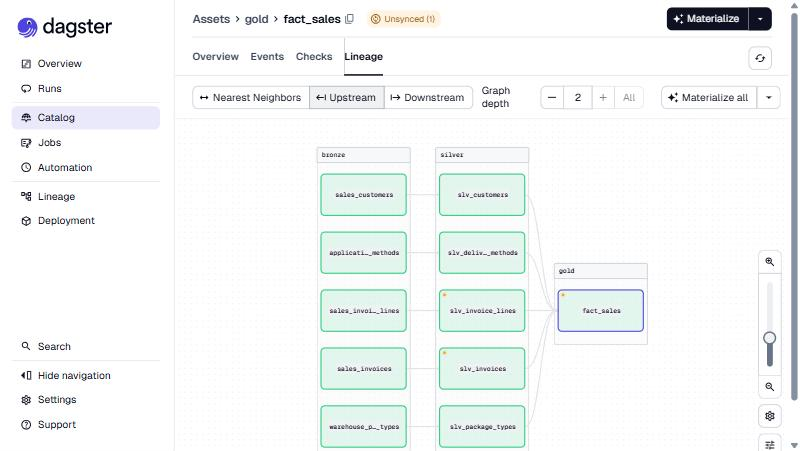
\includegraphics[width=0.92\linewidth]{figures/dagster_lineage.jpg}
\caption{Lignage amont de \texttt{gold/fact\_sales} dans Dagster (Bronze $\rightarrow$ Silver $\rightarrow$ Gold)}
\label{fig:lineage}
\end{figure}

\subsection{Planification et reprise sur erreur}
Le job \texttt{wwi\_daily\_job} rejoue toute la chaîne : ingestion DLT, puis \texttt{dbt build}. Il est
déclenché \textbf{chaque jour à 06\,h\,00 (heure de Dakar)} par le planning
\texttt{wwi\_daily\_schedule}. Une politique de reprise (\texttt{RetryPolicy}) relance automatiquement
une étape en échec jusqu'à deux fois, à 60 secondes d'intervalle, ce qui absorbe les erreurs
transitoires (réseau, verrou temporaire).

\begin{figure}[H]
\centering
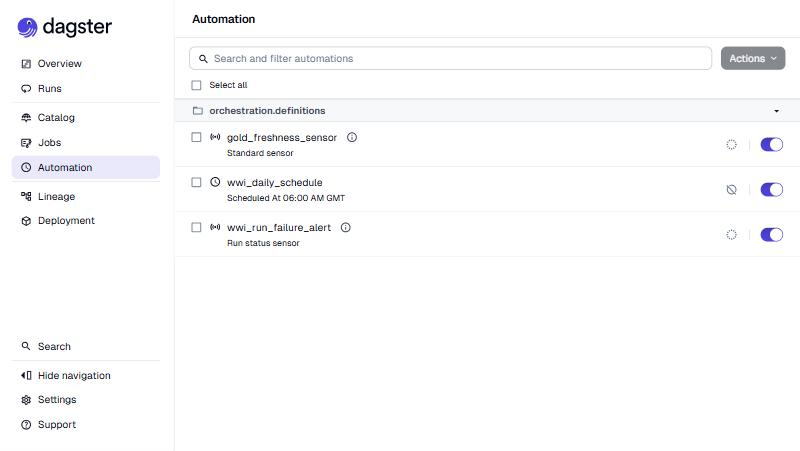
\includegraphics[width=0.85\linewidth]{figures/dagster_automation.jpg}
\caption{Automatisations actives dans Dagster : planning quotidien et capteurs d'alerte}
\label{fig:automation}
\end{figure}

Le premier run complet du job a réussi en environ 4\,min\,30 (3\,min\,32 pour l'étape Bronze, 53 s
pour l'étape dbt).

\chapter{Application Text-to-SQL avec Cortex AI}
\label{ch:application}

\section{Choix du service : Cortex Analyst}

Deux approches étaient envisageables pour générer le SQL avec Snowflake Cortex :
\begin{enumerate}
  \item appeler une fonction LLM générique (\texttt{SNOWFLAKE.CORTEX.COMPLETE}) en lui fournissant la
        question et une description textuelle du schéma ;
  \item utiliser \textbf{Cortex Analyst}, service spécialisé guidé par un modèle sémantique.
\end{enumerate}

Les tests réalisés sur le compte ont tranché la question : sur un \textbf{compte d'essai} Snowflake,
toutes les fonctions LLM génériques (\texttt{COMPLETE}, \texttt{AI\_COMPLETE}, \texttt{SENTIMENT},
\texttt{AI\_CLASSIFY}\ldots) sont désactivées et renvoient l'erreur
« \emph{AI function \ldots{} is not available for trial accounts} ». Cortex Analyst, en revanche, est
disponible. Ce choix est par ailleurs le plus pertinent techniquement : le modèle sémantique encode la
connaissance métier (synonymes, calculs, jointures) et produit un SQL nettement plus fiable qu'une
génération libre.

\section{Le modèle sémantique}

Le fichier \texttt{app/semantic\_model.yaml} décrit la couche Gold pour Cortex Analyst :
\begin{itemize}
  \item \textbf{10 tables logiques} (5 faits, 5 dimensions), chacune avec ses dimensions, dimensions
        temporelles, faits et métriques ;
  \item \textbf{des synonymes français} : « CA », « chiffre d'affaires », « ventes » pour
        \texttt{amount\_excluding\_tax} ; « marge », « bénéfice » pour \texttt{profit} ;
        « commercial », « vendeur » pour \texttt{employee\_name}\ldots ;
  \item \textbf{des valeurs d'exemple} (\texttt{sample\_values}) relevées dans les données réelles, qui
        aident le modèle à traduire « supermarchés » en \texttt{'Supermarket'} ;
  \item \textbf{des métriques} : chiffre d'affaires total, bénéfice total, taux de marge, nombre de
        factures et de commandes ;
  \item \textbf{11 relations} de type plusieurs-à-un entre faits et dimensions ;
  \item \textbf{3 requêtes vérifiées} correspondant aux questions de l'énoncé ;
  \item \textbf{des instructions personnalisées} : répondre en français, considérer par défaut le CA hors
        taxes, limiter les classements à 10 lignes, arrondir à deux décimales.
\end{itemize}

\begin{lstlisting}[language=yaml, caption={Extrait du modèle sémantique : table des ventes et métrique de marge}, label=lst:semantic]
- name: fact_sales
  description: Ventes facturées, une ligne par ligne de facture.
  base_table: {database: WWI_DB, schema: GOLD, table: FACT_SALES}
  primary_key: {columns: [invoice_line_id]}
  time_dimensions:
    - {name: invoice_date, expr: invoice_date, data_type: date,
       synonyms: [date de vente, date de facture, date]}
  facts:
    - {name: amount_excluding_tax, expr: amount_excluding_tax, data_type: number,
       synonyms: [chiffre d'affaires, CA, ventes, revenu, montant HT]}
    - {name: profit, expr: profit, data_type: number, synonyms: [bénéfice, marge, profit]}
  metrics:
    - {name: margin_rate, expr: "SUM(profit) / NULLIF(SUM(amount_excluding_tax), 0)",
       description: Taux de marge (bénéfice / CA HT), synonyms: [taux de marge]}
\end{lstlisting}

\begin{infobox}[title=Point d'attention rencontré]
Dans la syntaxe YAML compacte \texttt{\{clé: valeur, \ldots\}}, une virgule non protégée termine la
valeur. L'expression \texttt{NULLIF(SUM(\ldots), 0)} était ainsi tronquée et Cortex Analyst rejetait le
modèle (« \emph{Invalid semantic model yaml} »). Toute expression contenant une virgule doit être placée
entre guillemets.
\end{infobox}

\section{Fonctionnement de l'application}

La figure~\ref{fig:sequence} décrit le traitement d'une question.

\begin{figure}[H]
\centering
\resizebox{\linewidth}{!}{%
\begin{tikzpicture}[
  actor/.style={draw, rounded corners=3pt, fill=ucadblue!12, font=\footnotesize\bfseries, minimum width=2.6cm, minimum height=0.8cm},
  msg/.style={-{Stealth[length=2.2mm]}, thick},
  ret/.style={-{Stealth[length=2.2mm]}, thick, dashed},
  note/.style={font=\scriptsize, fill=white, inner sep=1.5pt}]
  \node[actor] (u) at (0,0) {Décideur};
  \node[actor] (st) at (4.2,0) {Streamlit};
  \node[actor, fill=snow!20] (ca) at (8.8,0) {Cortex Analyst};
  \node[actor, fill=gold!30] (g) at (13.2,0) {Snowflake GOLD};
  \foreach \n in {u,st,ca,g} \draw[black!30] (\n.south) -- ++(0,-6.4);
  \draw[msg] (0,-0.9) -- node[note, above]{« Quels produits génèrent le plus de bénéfices ? »} (4.2,-0.9);
  \draw[msg] (4.2,-1.7) -- node[note, above]{question + historique + modèle sémantique} (8.8,-1.7);
  \draw[ret] (8.8,-2.5) -- node[note, above]{interprétation + requête SQL} (4.2,-2.5);
  \draw[msg] (4.2,-3.1) -- ++(0.9,0) |- node[note, right, pos=0.25]{contrôle lecture seule} (4.25,-3.7);
  \draw[msg] (4.2,-4.4) -- node[note, above]{exécution (rôle \texttt{WWI\_ANALYST})} (13.2,-4.4);
  \draw[ret] (13.2,-5.2) -- node[note, above]{résultats} (4.2,-5.2);
  \draw[ret] (4.2,-6.0) -- node[note, above]{interprétation, SQL, graphique, tableau, CSV} (0,-6.0);
\end{tikzpicture}}
\caption{Traitement d'une question en langage naturel}
\label{fig:sequence}
\end{figure}

\subsection{Architecture du code}
Le code est séparé en deux modules :
\begin{itemize}
  \item \texttt{cortex\_analyst.py} : le \emph{moteur}, indépendant de l'interface. Il envoie la
        conversation à Cortex Analyst, contrôle et exécute le SQL. Il propose deux implémentations
        interchangeables : \texttt{LocalBackend} (connecteur Python et identifiants du fichier
        \texttt{.env}) et \texttt{SnowflakeBackend} (session active de Streamlit in Snowflake, sans
        identifiant à gérer) ;
  \item \texttt{streamlit\_app.py} : l'\emph{interface} de conversation.
\end{itemize}

\subsection{Conversation multi-tours}
L'historique complet des échanges est transmis à Cortex Analyst à chaque question. Les questions de
suivi sont ainsi interprétées dans leur contexte : après « Quel est le chiffre d'affaires par catégorie
de client et par année ? », la question « Et seulement pour les supermarchés, par mois en 2015 ? » est
correctement comprise comme « \emph{le chiffre d'affaires HT par mois en 2015, uniquement pour la
catégorie de client Supermarket} ».

\subsection{Choix automatique de la visualisation}
L'application analyse le résultat pour choisir la représentation la plus adaptée :
\begin{itemize}
  \item une valeur unique est affichée comme un \textbf{indicateur} (KPI) ;
  \item si une colonne est temporelle (date, mois, année\ldots), une \textbf{courbe} est tracée, avec une
        série par catégorie si une seconde dimension est présente ;
  \item sinon, un \textbf{diagramme en barres} horizontal trié par valeur décroissante est affiché.
\end{itemize}
Les colonnes numériques représentant le temps (année, mois) ou des identifiants sont traitées comme des
axes et non comme des mesures.

\section{Sécurité de la génération de SQL}

Confier l'écriture du SQL à un modèle de langage impose des garde-fous. Trois niveaux de protection se
cumulent :
\begin{enumerate}
  \item \textbf{Contrôle syntaxique} avant exécution (listing~\ref{lst:guard}) : une seule instruction,
        commençant par \texttt{SELECT} ou \texttt{WITH}, sans aucun mot-clé d'écriture ou
        d'administration ;
  \item \textbf{Moindre privilège} : la requête est exécutée avec le rôle \texttt{WWI\_ANALYST}, qui ne
        peut que lire le schéma Gold ;
  \item \textbf{Limitation des volumes} : 10\,000 lignes au maximum sont rapatriées.
\end{enumerate}

\begin{lstlisting}[language=Python, caption={Contrôle de lecture seule du SQL généré}, label=lst:guard]
FORBIDDEN = re.compile(
    r"\b(insert|update|delete|merge|drop|create|alter|truncate|grant|revoke"
    r"|call|copy|put|remove|use|execute)\b", re.IGNORECASE)

def check_read_only(sql: str) -> None:
    """Refuse toute requête qui n'est pas une simple lecture."""
    stripped = re.sub(r"--[^\n]*|/\*.*?\*/", "", sql, flags=re.DOTALL).strip().rstrip(";")
    if ";" in stripped:
        raise ValueError("Une seule instruction SQL est autorisée.")
    if not re.match(r"^(with|select)\b", stripped, re.IGNORECASE):
        raise ValueError("Seules les requêtes SELECT sont autorisées.")
    if FORBIDDEN.search(stripped):
        raise ValueError("La requête contient une instruction non autorisée.")
\end{lstlisting}

\section{Interface utilisateur}

L'interface reprend l'identité visuelle de l'Université Cheikh Anta Diop : un en-tête présente le logo,
le nom de l'université et de la faculté, et un pied de page rappelle le département, la section et la
formation. La barre latérale propose des questions d'exemple et la réinitialisation de la conversation.

\begin{figure}[H]
\centering

\includegraphics[width=0.88\linewidth]{figures/app_accueil.jpg}
\caption{Page d'accueil de l'application : en-tête UCAD, exemples de questions et pied de page}
\label{fig:app-accueil}
\end{figure}

\begin{figure}[H]
\centering
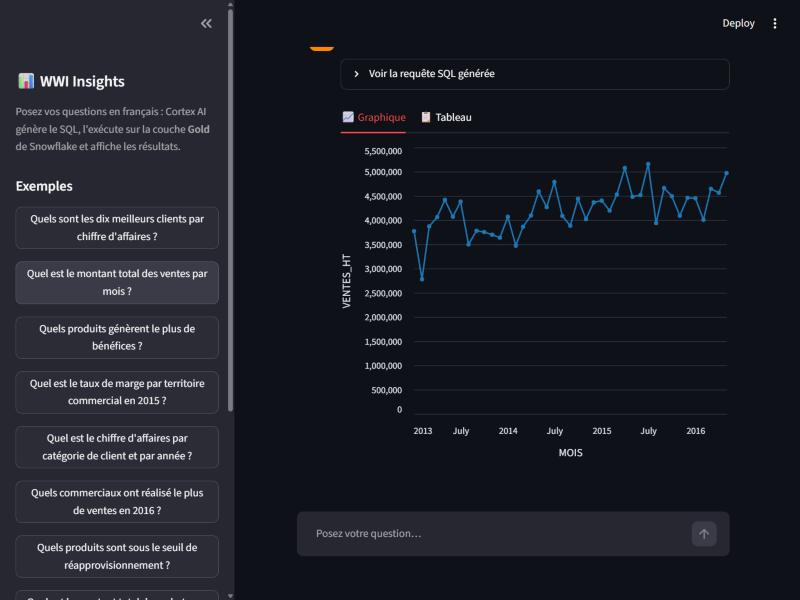
\includegraphics[width=0.88\linewidth]{figures/app_ventes_mois.jpg}
\caption{« Quel est le montant total des ventes par mois ? » : courbe générée automatiquement}
\label{fig:app-mois}
\end{figure}

\begin{figure}[H]
\centering
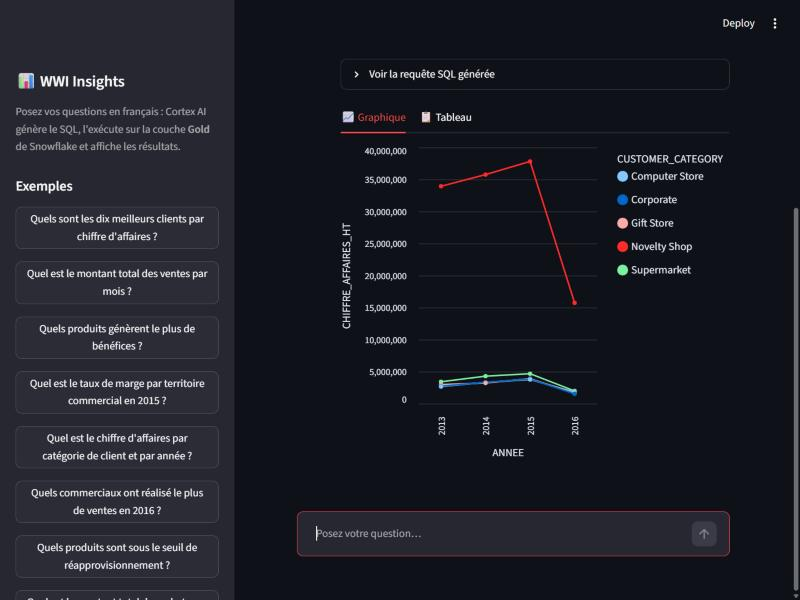
\includegraphics[width=0.88\linewidth]{figures/app_categorie_annee.jpg}
\caption{« Quel est le chiffre d'affaires par catégorie de client et par année ? » : une série par catégorie}
\label{fig:app-categorie}
\end{figure}

Pour chaque réponse, l'utilisateur dispose de l'interprétation de sa question par Cortex Analyst, de la
requête SQL générée (dans un panneau dépliable, pour la transparence et l'apprentissage), du graphique,
du tableau de résultats et d'un export CSV. En cas d'ambiguïté, Cortex Analyst propose des
reformulations cliquables.

\chapter{Industrialisation de la plateforme}
\label{ch:industrialisation}

Une fois la chaîne fonctionnelle, plusieurs limites ont été identifiées : absence d'historique,
reconstruction complète de toutes les tables à chaque exécution, application dépendante d'un poste
local, absence d'alerte en cas d'incident et validation manuelle des modifications. Ce chapitre présente
les réponses apportées. L'historisation ayant été décrite à la section~\ref{sec:scd2}, il traite les
quatre autres points.

\section{Traitements incrémentaux}
\label{sec:incremental}

Dans la version initiale, \texttt{dbt build} reconstruisait intégralement toutes les tables. Ce coût,
négligeable sur WWI, devient prohibitif sur des volumes réels. Les \textbf{dix modèles les plus
volumineux} sont désormais matérialisés en mode \texttt{incremental} avec la stratégie \texttt{merge}
(tableau~\ref{tab:incremental}).

\begin{table}[H]
\centering
\caption{Modèles incrémentaux}
\label{tab:incremental}
\begin{tabular}{@{}l l l@{}}
\toprule
\textbf{Couche} & \textbf{Modèle} & \textbf{Clé de fusion} \\
\midrule
\multirow{6}{*}{Silver} & \texttt{slv\_invoice\_lines} & \texttt{invoice\_line\_id} \\
 & \texttt{slv\_invoices} & \texttt{invoice\_id} \\
 & \texttt{slv\_order\_lines} & \texttt{order\_line\_id} \\
 & \texttt{slv\_orders} & \texttt{order\_id} \\
 & \texttt{slv\_stock\_item\_transactions} & \texttt{stock\_item\_transaction\_id} \\
 & \texttt{slv\_customer\_transactions} & \texttt{customer\_transaction\_id} \\
\midrule
\multirow{4}{*}{Gold} & \texttt{fact\_sales} & \texttt{invoice\_line\_id} \\
 & \texttt{fact\_orders} & \texttt{order\_line\_id} \\
 & \texttt{fact\_stock\_movements} & \texttt{stock\_item\_transaction\_id} \\
 & \texttt{fact\_customer\_transactions} & \texttt{customer\_transaction\_id} \\
\bottomrule
\end{tabular}
\end{table}

Une macro \texttt{incremental\_filter} ne retient que les lignes dont la date de dernière modification
est postérieure à la plus récente déjà présente dans la table cible. Pour les faits issus d'une jointure
en-tête/ligne, la date retenue est la plus récente des deux (\texttt{GREATEST}), de sorte qu'une
modification de l'en-tête (par exemple la date de livraison d'une facture) est aussi propagée.

\begin{resultbox}[title=Vérification]
Après une reconstruction complète (\texttt{dbt build -{}-full-refresh}), une exécution normale des dix
modèles incrémentaux a traité \textbf{0 ligne} au lieu de 228\,265 pour \texttt{fact\_sales} : seules les
modifications seront désormais retraitées.
\end{resultbox}

\section{Alertes et supervision}

\subsection{Alertes Dagster}
Le module \texttt{orchestration/alerts.py} ajoute deux capteurs actifs par défaut :
\begin{itemize}
  \item \texttt{wwi\_run\_failure\_alert} : un \emph{run failure sensor} déclenché dès qu'un run échoue.
        Il construit un message (job, identifiant du run, étapes en échec, erreur, lien vers
        l'interface) et l'envoie sur \textbf{Slack} (webhook) et/ou par \textbf{e-mail} (SMTP) selon
        la configuration du fichier \texttt{.env} ; à défaut, l'alerte est journalisée ;
  \item \texttt{gold\_freshness\_sensor} : des \textbf{contrôles de fraîcheur} vérifient que les tables
        Gold principales ont été rafraîchies au cours des 26 dernières heures (exécution quotidienne
        plus une marge de deux heures). Un planning bloqué ou un démon arrêté est ainsi détecté.
\end{itemize}

\subsection{Maîtrise des coûts Snowflake}
Un \textbf{moniteur de ressources} (\texttt{WWI\_CREDIT\_MONITOR}) est associé à l'entrepôt
\texttt{WWI\_WH} : il envoie une notification à 75\,\% et 90\,\% du quota mensuel de crédits, suspend
l'entrepôt à 100\,\% et l'arrête immédiatement à 110\,\%. Il protège en particulier les crédits limités
du compte d'essai.

\section{Déploiement dans Streamlit in Snowflake}

L'application, initialement exécutée sur le poste du développeur, a été rendue déployable dans
\textbf{Streamlit in Snowflake}. Ce mode d'hébergement présente plusieurs avantages :
\begin{itemize}
  \item aucun serveur ni identifiant à gérer : l'application utilise la session de l'utilisateur
        connecté à Snowsight ;
  \item les données ne quittent pas Snowflake ;
  \item le partage se fait par les mécanismes de droits de Snowflake.
\end{itemize}

Le script \texttt{deploy/deploy\_sis.py} automatise le déploiement :
\begin{enumerate}
  \item création du schéma \texttt{WWI\_DB.APP} et attribution au rôle \texttt{WWI\_ANALYST} des droits
        de création de stage et d'application ;
  \item création d'un stage interne et envoi des fichiers de l'application (\texttt{PUT}) : code,
        modèle sémantique, logo et fichier \texttt{environment.yml} des dépendances ;
  \item création de l'objet \texttt{STREAMLIT WWI\_DB.APP.WWI\_INSIGHTS} avec l'entrepôt
        \texttt{WWI\_WH}.
\end{enumerate}

L'application appartient au rôle \texttt{WWI\_ANALYST} : elle s'exécute donc avec ses seuls droits de
lecture sur Gold. Le même code source fonctionne dans les deux environnements, le moteur détectant la
présence du module interne \texttt{\_snowflake} pour choisir entre l'appel REST local et l'API interne
\texttt{\_snowflake.send\_snow\_api\_request}.

\section{Intégration et déploiement continus}

Le dépôt est hébergé sur GitHub. Le workflow \texttt{.github/workflows/ci.yml} s'exécute à chaque
\emph{push} et à chaque \emph{pull request} (figure~\ref{fig:ci}).

\begin{figure}[H]
\centering
\resizebox{\linewidth}{!}{%
\begin{tikzpicture}[node distance=1.1cm]
  \node[box, fill=gray!10] (push) {\textbf{push / PR}\\ GitHub};
  \node[box, fill=blue!8, right=of push, text width=3.3cm] (q) {\textbf{Qualité}\\ \scriptsize ruff, compilation,\\ validation YAML};
  \node[box, fill=snow!15, right=of q, text width=3.5cm] (d) {\textbf{dbt build}\\ \scriptsize sur clone zéro copie\\ \texttt{WWI\_DB\_CI\_<run>}};
  \node[box, fill=green!10, right=of d, text width=3.3cm] (dep) {\textbf{Déploiement}\\ \scriptsize Streamlit in Snowflake\\ (branche \texttt{main})};
  \draw[flow] (push) -- (q);
  \draw[flow] (q) -- (d);
  \draw[flow] (d) -- (dep);
  \node[below=0.35cm of d, font=\scriptsize, text width=4.5cm, align=center] {le clone est supprimé à la fin,\\ même en cas d'échec};
\end{tikzpicture}}
\caption{Chaîne d'intégration et de déploiement continus}
\label{fig:ci}
\end{figure}

\begin{enumerate}
  \item \textbf{Qualité} : analyse statique du code Python (\texttt{ruff}), compilation de tous les
        scripts, validation syntaxique de tous les fichiers YAML et de la structure du modèle sémantique.
  \item \textbf{dbt} : la base de production est clonée par \textbf{clonage zéro copie}
        (\texttt{CREATE DATABASE WWI\_DB\_CI\_<run> CLONE WWI\_DB}) : le clone est instantané et ne
        duplique aucune donnée. \texttt{dbt build} y est exécuté (modèles, snapshot et tests), puis le
        clone est supprimé. Les modifications sont ainsi testées sur des données réelles sans jamais
        toucher à la production. La base cible étant paramétrée par la variable
        \texttt{SNOWFLAKE\_DATABASE}, aucun code n'est spécifique à la CI.
  \item \textbf{Déploiement} : sur la branche \texttt{main}, si les étapes précédentes réussissent,
        l'application Streamlit in Snowflake est redéployée.
\end{enumerate}

Les identifiants Snowflake sont stockés dans les \emph{secrets} chiffrés du dépôt GitHub, jamais dans
le code.

\chapter{Résultats et évaluation}
\label{ch:resultats}

\section{Bilan quantitatif de la plateforme}

\begin{table}[H]
\centering
\caption{Indicateurs de la plateforme réalisée}
\label{tab:bilan}
\begin{tabularx}{\linewidth}{@{}X r@{}}
\toprule
\textbf{Élément} & \textbf{Valeur} \\
\midrule
Tables ingérées en Bronze (dont 2 tables d'archive) & 30 \\
Lignes chargées (premier chargement) & $\approx$ 1 million \\
Modèles Silver / snapshot & 29 / 1 \\
Tables Gold (dimensions, faits, historisation) & 15 \\
Nœuds dbt exécutés par \texttt{dbt build} (modèles, snapshot, tests) & 189 \\
Tests dbt (tous au vert) & 144 \\
Assets Dagster / contrôles de qualité & 75 / 146 \\
Écart de volume SQL Server / Bronze & 0 ligne \\
Écart de CA TTC Bronze / Gold & 0 \\
Durée d'une exécution complète (ingestion + dbt) & $\approx$ 4 min 30 \\
Lignes retraitées par une exécution incrémentale sans changement & 0 \\
\bottomrule
\end{tabularx}
\end{table}

\section{Évaluation de l'application Text-to-SQL}

Un script de test de bout en bout (\texttt{app/test\_questions.py}) soumet une série de questions à
Cortex Analyst, exécute le SQL obtenu et affiche les résultats. Les réponses ont été comparées à des
requêtes SQL écrites manuellement : \textbf{toutes les questions testées ont produit un SQL exécutable
et des résultats identiques} à la référence (tableau~\ref{tab:eval}).

\begin{longtable}{@{}p{6.2cm}p{8.3cm}@{}}
\caption{Questions testées et résultats obtenus}
\label{tab:eval}\\
\toprule
\textbf{Question posée en français} & \textbf{Résultat (extrait)} \\
\midrule
\endfirsthead
\toprule
\textbf{Question posée en français} & \textbf{Résultat (extrait)} \\
\midrule
\endhead
Quels sont les dix meilleurs clients par chiffre d'affaires ? &
  1\textsuperscript{er} : Tailspin Toys (Inguadona, MN) avec 381\,585,35~\$ HT ; puis Tailspin Toys
  (Minidoka, ID) avec 371\,822,30~\$ et Mauno Laurila avec 369\,058,30~\$. \\
\addlinespace
Quel est le montant total des ventes par mois ? &
  41 mois, de janvier 2013 (3\,770\,410,85~\$) à mai 2016 ; courbe affichée automatiquement. \\
\addlinespace
Quels produits génèrent le plus de bénéfices ? &
  « 20 mm Double sided bubble wrap 50m » : 5\,293\,680~\$ ; « Air cushion machine (Blue) » :
  4\,439\,391~\$. \\
\addlinespace
Quel est le taux de marge par territoire commercial en 2015 ? &
  9 territoires ; de 50,57~\% (Great Lakes) à environ 49,9~\% ; utilisation de la métrique
  \texttt{margin\_rate}. \\
\addlinespace
Quels produits sont sous le seuil de réapprovisionnement ? &
  2 produits, dont « Shipping carton (Brown) 305x305x305mm » (38 unités pour un seuil de 50). \\
\addlinespace
Quel est le chiffre d'affaires par pays ? &
  United States : 172\,261\,341,20~\$ HT (tous les clients de WWI sont américains). \\
\addlinespace
Quel est le chiffre d'affaires par catégorie de client et par année ? &
  Novelty Shop domine chaque année (environ 38 M\$ en 2015) ; une série par catégorie. \\
\addlinespace
\emph{(suivi)} Et seulement pour les supermarchés, par mois en 2015 ? &
  Question interprétée dans le contexte : CA HT mensuel 2015 de la catégorie \texttt{Supermarket}. \\
\bottomrule
\end{longtable}

\section{Quelques enseignements métier}

Les données de la couche Gold permettent de dégager rapidement une vue d'ensemble de l'activité de
Wide World Importers :
\begin{itemize}
  \item un chiffre d'affaires cumulé de \textbf{172,3 M\$ HT} sur 70\,510 factures, pour un bénéfice de
        \textbf{85,7 M\$}, soit un taux de marge d'environ \textbf{49,8~\%} ;
  \item une croissance régulière du CA : 45,7 M\$ en 2013, 49,9 M\$ en 2014 et 54,0 M\$ en 2015
        (l'année 2016 ne couvre que cinq mois) ;
  \item un taux de marge très homogène entre territoires commerciaux (entre 49,9~\% et 50,6~\% en 2015) ;
  \item une forte concentration des achats sur deux fournisseurs (Fabrikam, Inc. et Litware, Inc.).
\end{itemize}

\begin{infobox}[title=Remarque sur les données]
Dans WWI, le montant total des achats fournisseurs (environ 946 M\$, cohérent avec les factures
fournisseurs de la source : 944 M\$) dépasse largement le chiffre d'affaires. Il s'agit d'une
caractéristique connue de ce jeu de données synthétique, et non d'une erreur de transformation. De même,
la plupart des versions archivées des produits datent de la fin de la période (31 mai 2016) et
correspondent à des mises à jour techniques : le mécanisme d'historisation est en place et sera
pleinement exploité sur des données réelles.
\end{infobox}

\section{Difficultés rencontrées et solutions}

\begin{longtable}{@{}p{5.6cm}p{8.9cm}@{}}
\caption{Principales difficultés et solutions apportées}
\label{tab:difficultes}\\
\toprule
\textbf{Difficulté} & \textbf{Solution} \\
\midrule
\endfirsthead
\toprule
\textbf{Difficulté} & \textbf{Solution} \\
\midrule
\endhead
Accès refusé du service SQL Server au fichier de sauvegarde &
  Copie du \texttt{.bak} dans un dossier partagé lisible par le compte de service. \\
\addlinespace
Certificat non approuvé avec le pilote ODBC 18 &
  Option \texttt{TrustServerCertificate} (\texttt{-C}) pour l'instance locale. \\
\addlinespace
Épuisement du pool de connexions SQLAlchemy lors de l'extraction parallèle &
  Utilisation d'un \texttt{NullPool} (une connexion par table extraite). \\
\addlinespace
Types \texttt{geography} et \texttt{varbinary} non transférables &
  Exclusion des colonnes avant extraction (\texttt{table\_adapter\_callback}). \\
\addlinespace
Risque de perte de données : table sans clé chargée en mode incrémental \texttt{replace} &
  Incrémental activé uniquement pour les tables dotées d'une clé primaire ; tables d'archive en
  rechargement complet. \\
\addlinespace
Fonctions LLM de Cortex indisponibles sur un compte d'essai &
  Recours à Cortex Analyst et à un modèle sémantique, solution par ailleurs plus fiable. \\
\addlinespace
Modèle sémantique rejeté (expression tronquée par une virgule en YAML) &
  Mise entre guillemets des expressions contenant une virgule ; validation YAML ajoutée en CI. \\
\addlinespace
Graphique erroné : l'année, numérique, prise pour une mesure &
  Les colonnes temporelles et les identifiants sont traités comme des axes. \\
\addlinespace
\texttt{dbt} introuvable par Dagster lorsque l'environnement virtuel n'est pas activé &
  Ajout du dossier de l'environnement virtuel au \texttt{PATH} au chargement des définitions. \\
\bottomrule
\end{longtable}

\section{Limites}

\begin{itemize}
  \item Le compte Snowflake est un compte d'essai (30 jours, 400~\$ de crédits) : les fonctions LLM
        génériques n'y sont pas disponibles.
  \item Le système source est une instance SQL Server locale : en production, l'ingestion serait
        exécutée sur un serveur ou un conteneur ayant accès à la source et à Snowflake.
  \item La qualité de la génération SQL dépend du modèle sémantique ; les questions portant sur des
        notions non décrites (par exemple les températures des entrepôts frigorifiques, non ingérées)
        ne peuvent pas recevoir de réponse.
  \item L'exécution de la CI sur la base clonée suppose l'octroi préalable du privilège
        \texttt{CREATE DATABASE} au rôle \texttt{WWI\_ENGINEER} (script
        \texttt{snowflake/01\_ameliorations.sql}).
\end{itemize}

\chapter*{Conclusion générale et perspectives}
\addcontentsline{toc}{chapter}{Conclusion générale et perspectives}
\markboth{Conclusion générale et perspectives}{}

Ce projet avait pour objectif de concevoir une Modern Data Platform capable d'automatiser l'ingestion,
la transformation et la modélisation des données, et d'offrir aux décideurs une interface leur
permettant d'interroger ces données en langage naturel.

Cet objectif est atteint. Les données transactionnelles de Wide World Importers sont extraites de
SQL Server par \textbf{DLT} de manière incrémentale et chargées dans \textbf{Snowflake}, où elles sont
organisées selon une \textbf{architecture Médaillon}. La couche Bronze conserve une copie fidèle et
réconciliée de la source ; la couche Silver applique des règles de nettoyage homogènes et factorisées ;
la couche Gold expose un schéma en étoile complété de dimensions historisées en SCD de type 2. Les
transformations, développées avec \textbf{dbt}, sont versionnées, documentées et couvertes par plus de
140 tests. L'ensemble est orchestré par \textbf{Dagster}, qui offre un lignage de bout en bout, une
exécution quotidienne avec reprise automatique, des contrôles de fraîcheur et des alertes.

L'application \textbf{Streamlit}, adossée à \textbf{Snowflake Cortex Analyst} et à un modèle sémantique
riche, répond correctement aux questions de l'énoncé et à des questions plus élaborées, y compris des
questions de suivi, en restituant le SQL généré, un graphique adapté et le tableau des résultats. Sa
conception place la sécurité au premier plan : contrôle de lecture seule, rôle aux droits minimaux et
absence d'identifiants dans le code. Déployée aussi dans \textbf{Streamlit in Snowflake} et validée par
une chaîne d'\textbf{intégration continue} sur clone zéro copie, la plateforme dépasse le stade du
prototype pour s'approcher d'une solution industrialisée.

Sur le plan personnel, ce projet m'a permis de mettre en pratique l'ensemble de la chaîne de valeur de
la donnée --- ingénierie, modélisation dimensionnelle, qualité, orchestration, sécurité, DevOps --- et
de mesurer l'apport, mais aussi les exigences, de l'intelligence artificielle générative appliquée à
l'analyse de données : un LLM n'est fiable que s'il s'appuie sur un modèle de données propre et sur
une sémantique métier explicitement décrite.

\section*{Perspectives}

Plusieurs prolongements sont envisageables :
\begin{itemize}
  \item \textbf{Enrichissement du modèle sémantique} : nouvelles requêtes vérifiées issues des questions
        réelles des utilisateurs, publication sous forme de \emph{semantic view} Snowflake, et
        couverture des historisations SCD2 et des températures d'entrepôt ;
  \item \textbf{Retour utilisateur} : collecte des appréciations (réponse correcte ou non) pour mesurer
        en continu la précision du Text-to-SQL ;
  \item \textbf{Ingestion en quasi temps réel} : exploitation de la capture des changements (CDC) de
        SQL Server ou d'un ordonnancement plus fréquent ;
  \item \textbf{Gouvernance} : masquage dynamique des données personnelles, politiques d'accès par ligne
        (\emph{row access policies}) selon le territoire commercial de l'utilisateur, catalogue de
        données ;
  \item \textbf{Observabilité} : tableau de bord de suivi des coûts Snowflake, des durées d'exécution et
        des résultats des tests ;
  \item \textbf{Restitution} : tableaux de bord prédéfinis (Power BI, Streamlit) pour les indicateurs
        récurrents, l'interface conversationnelle restant dédiée aux questions ad hoc.
\end{itemize}


\appendix
\chapter{Structure du dépôt}
\label{ann:depot}

Le code source est disponible sur GitHub :

\url{https://github.com/mouhameddiop06/wwi-modern-data-platform}.

\begin{lstlisting}[language={}, numbers=none, caption={Arborescence du projet}]
projet_pratique_bi/
|-- .env.example              Modèle des paramètres de connexion
|-- requirements.txt          Dépendances Python
|-- pyproject.toml            Configuration du lint (ruff)
|-- dbt.ps1 / dagster.ps1 / streamlit.ps1   Scripts de lancement
|-- snowflake/
|   |-- 00_setup.sql          Entrepôt, base, schémas, rôles, utilisateur
|   `-- 01_ameliorations.sql  Moniteur de crédits, droits CI, schéma APP
|-- ingestion/
|   |-- wwi_pipeline.py       Pipeline DLT SQL Server -> BRONZE
|   `-- check_bronze.py       Réconciliation des volumes
|-- transform/wwi_dbt/
|   |-- dbt_project.yml, profiles.yml
|   |-- macros/               clean_text, to_amount, dedup, surrogate_key,
|   |                         incremental_filter, generate_schema_name
|   |-- models/silver/        29 modèles slv_* + sources
|   |-- models/gold/          dimensions, faits, historisation + tests
|   |-- snapshots/            snapshot du niveau de stock
|   `-- tests/                tests métier personnalisés
|-- orchestration/
|   |-- definitions.py        Assets DLT + dbt, job, planning
|   `-- alerts.py             Alertes d'échec et contrôles de fraîcheur
|-- app/
|   |-- streamlit_app.py      Interface utilisateur
|   |-- cortex_analyst.py     Moteur Text-to-SQL (local / Snowflake)
|   |-- semantic_model.yaml   Modèle sémantique de la couche GOLD
|   |-- environment.yml       Dépendances Streamlit in Snowflake
|   `-- test_questions.py     Test de bout en bout
|-- deploy/deploy_sis.py      Déploiement Streamlit in Snowflake
|-- ci/snowflake_clone.py     Clone zéro copie pour la CI
|-- .github/workflows/ci.yml  Intégration et déploiement continus
`-- rapport/                  Ce rapport (LaTeX)
\end{lstlisting}

\chapter{Guide d'installation et commandes}
\label{ann:commandes}

\section*{Installation}
\begin{enumerate}
  \item Restaurer \texttt{WideWorldImporters-Full.bak} dans SQL Server (2016 SP1 ou ultérieur).
  \item Créer un compte Snowflake (édition Enterprise) et exécuter \texttt{snowflake/00\_setup.sql},
        puis \texttt{snowflake/01\_ameliorations.sql}, en \texttt{ACCOUNTADMIN}.
  \item Copier \texttt{.env.example} en \texttt{.env} et renseigner l'identifiant du compte et le mot de
        passe de l'utilisateur technique.
  \item Créer l'environnement Python : \texttt{python -m venv .venv}, puis
        \texttt{.venv\textbackslash Scripts\textbackslash python.exe -m pip install -r requirements.txt}.
\end{enumerate}

\section*{Commandes principales}
\begin{table}[H]
\centering
\small
\begin{tabularx}{\linewidth}{@{}X l@{}}
\toprule
\textbf{Objectif} & \textbf{Commande} \\
\midrule
Ingestion incrémentale Bronze & \texttt{python ingestion/wwi\_pipeline.py} \\
Rechargement complet & \texttt{python ingestion/wwi\_pipeline.py -{}-full-refresh} \\
Réconciliation des volumes & \texttt{python ingestion/check\_bronze.py} \\
Construire et tester Silver et Gold & \texttt{.\textbackslash dbt.ps1 build} \\
Documentation et lignage dbt & \texttt{.\textbackslash dbt.ps1 docs generate} \\
Interface Dagster et planning & \texttt{.\textbackslash dagster.ps1} (port 3000) \\
Application en local & \texttt{.\textbackslash streamlit.ps1} (port 8501) \\
Test des questions de référence & \texttt{python app/test\_questions.py} \\
Déploiement Streamlit in Snowflake & \texttt{python deploy/deploy\_sis.py} \\
\bottomrule
\end{tabularx}
\end{table}

\chapter{Extraits de code complémentaires}

\begin{lstlisting}[language=Python, caption={Assets Bronze : relier DLT et dbt dans le lignage Dagster}]
class BronzeTranslator(DagsterDltTranslator):
    def get_asset_spec(self, data: DltResourceTranslatorData) -> AssetSpec:
        spec = super().get_asset_spec(data)
        return spec.replace_attributes(
            key=AssetKey(["bronze", snake(data.resource.name)]),  # = clé des sources dbt
            deps=[],
            group_name="bronze",
            kinds={"dlt", "sqlserver", "snowflake"},
        )

@dlt_assets(dlt_source=wwi_source(), dlt_pipeline=make_pipeline(progress=None),
            name="wwi_bronze", dagster_dlt_translator=BronzeTranslator())
def bronze_assets(context: AssetExecutionContext, dlt: DagsterDltResource):
    yield from dlt.run(context=context)
\end{lstlisting}

\begin{lstlisting}[language=Python, caption={Job quotidien avec reprise sur erreur}]
wwi_daily_job = define_asset_job(
    name="wwi_daily_job",
    selection=AssetSelection.all(),
    op_retry_policy=RetryPolicy(max_retries=2, delay=60),  # reprise sur erreur
)
wwi_daily_schedule = ScheduleDefinition(
    name="wwi_daily_schedule", job=wwi_daily_job,
    cron_schedule="0 6 * * *", execution_timezone="Africa/Dakar",
    default_status=DefaultScheduleStatus.RUNNING,
)
\end{lstlisting}

\begin{lstlisting}[language=SQL, caption={Dimension produit historisée (SCD2)}]
select
    h.stock_item_version_id, h.stock_item_id,
    h.stock_item_name as product_name, h.unit_price, h.recommended_retail_price,
    h.valid_from,
    case when h.valid_to >= '9999-01-01' then null else h.valid_to end as valid_to,
    h.valid_to >= '9999-01-01' as is_current,
    row_number() over (partition by h.stock_item_id order by h.valid_from) as version_number
from {{ ref('slv_stock_items_history') }} h
\end{lstlisting}

\begin{lstlisting}[language=Python, caption={Appel de Cortex Analyst dans Streamlit in Snowflake}]
def ask(self, messages: list[dict]) -> AnalystAnswer:
    resp = _snowflake.send_snow_api_request(
        "POST", "/api/v2/cortex/analyst/message", {}, {},
        {"messages": messages, "semantic_model": SEMANTIC_MODEL},
        None, 120_000,
    )
    body = json.loads(resp["content"])
    if resp["status"] >= 400:
        raise RuntimeError(f"Cortex Analyst a répondu {resp['status']}")
    return parse_answer(body)
\end{lstlisting}


\begin{thebibliography}{99}
\addcontentsline{toc}{chapter}{Bibliographie et webographie}

\bibitem{kimball}
R.~Kimball, M.~Ross, \emph{The Data Warehouse Toolkit: The Definitive Guide to Dimensional Modeling},
3\textsuperscript{e} édition, Wiley, 2013.

\bibitem{inmon}
W.~H.~Inmon, \emph{Building the Data Warehouse}, 4\textsuperscript{e} édition, Wiley, 2005.

\bibitem{reis}
J.~Reis, M.~Housley, \emph{Fundamentals of Data Engineering}, O'Reilly Media, 2022.

\bibitem{medallion}
Databricks, \emph{What is a medallion architecture?}
\url{https://www.databricks.com/glossary/medallion-architecture}

\bibitem{wwi}
Microsoft, \emph{Wide World Importers sample databases for Microsoft SQL}.
\url{https://learn.microsoft.com/sql/samples/wide-world-importers-what-is}

\bibitem{snowflake}
Snowflake, \emph{Snowflake Documentation}. \url{https://docs.snowflake.com}

\bibitem{cortexanalyst}
Snowflake, \emph{Cortex Analyst} et \emph{Cortex Analyst semantic model specification}.
\url{https://docs.snowflake.com/en/user-guide/snowflake-cortex/cortex-analyst}

\bibitem{sis}
Snowflake, \emph{About Streamlit in Snowflake}.
\url{https://docs.snowflake.com/en/developer-guide/streamlit/about-streamlit}

\bibitem{dlt}
dltHub, \emph{dlt documentation --- SQL database source, incremental loading}.
\url{https://dlthub.com/docs}

\bibitem{dbt}
dbt Labs, \emph{dbt Developer Hub --- models, tests, snapshots, incremental models}.
\url{https://docs.getdbt.com}

\bibitem{dagster}
Dagster Labs, \emph{Dagster documentation --- software-defined assets, dagster-dbt, dagster-dlt}.
\url{https://docs.dagster.io}

\bibitem{streamlit}
Streamlit, \emph{Streamlit documentation}. \url{https://docs.streamlit.io}

\bibitem{texttosql}
J.~Li et al., \emph{Can LLM Already Serve as A Database Interface? A BIg Bench for Large-Scale
Database Grounded Text-to-SQLs (BIRD)}, NeurIPS, 2023.

\end{thebibliography}


\end{document}
